\documentclass[12pt,oneside,openany]{book}
% Professional thesis layout used because no university LaTeX template was present.
\usepackage[T1]{fontenc}
\usepackage[utf8]{inputenc}
\usepackage{newtxtext,newtxmath}
\usepackage[a4paper,margin=28mm,headheight=15pt]{geometry}
\usepackage{microtype}
\usepackage{setspace}
\usepackage{parskip}
\usepackage{booktabs}
\usepackage{longtable}
\usepackage{tabularx}
\usepackage{array}
\usepackage{multirow}
\usepackage{graphicx}
\usepackage{float}
\usepackage{caption}
\usepackage{subcaption}
\usepackage{xcolor}
\usepackage{amsmath}
\usepackage{enumitem}
\usepackage{listings}
\usepackage{fancyhdr}
\usepackage{titlesec}
\usepackage{tikz}
\usetikzlibrary{arrows.meta,positioning,fit,calc,shapes.geometric,shapes.multipart,matrix,backgrounds}
\usepackage{pgfplots}
\pgfplotsset{compat=1.18}
\usepackage{cite}
\usepackage{url}
\usepackage[hidelinks,bookmarksnumbered=true,bookmarksopen=true,pdfdisplaydoctitle=true]{hyperref}
\usepackage[nameinlink,noabbrev]{cleveref}

\definecolor{Navy}{HTML}{16324F}
\definecolor{Blue}{HTML}{2266A5}
\definecolor{Teal}{HTML}{168C86}
\definecolor{Gold}{HTML}{C98B2E}
\definecolor{Slate}{HTML}{526273}
\definecolor{PaleBlue}{HTML}{EAF2F8}
\definecolor{PaleTeal}{HTML}{E7F5F2}
\definecolor{PaleGold}{HTML}{FBF3E3}
\definecolor{Warn}{HTML}{A33A2B}
\definecolor{CodeBg}{HTML}{F5F7F9}

\hypersetup{
  colorlinks=true,
  linkcolor=Navy,
  citecolor=Blue,
  urlcolor=Blue,
  pdftitle={Source-Traceable Research Intelligence: Evidence-Grounded Discovery, Question Answering, and Thesis-Extension Support},
  pdfauthor={Jarod Esareesingh},
  pdfsubject={MSc Data Science project, Department of Computing \& Information Technology, The University of the West Indies},
  pdfkeywords={research intelligence, information retrieval, retrieval-augmented generation, scholarly recommendation, responsible AI, reproducibility}
}

\onehalfspacing
\setlength{\parindent}{0pt}
\setlength{\parskip}{0.55em}
\setlength{\emergencystretch}{3em}
\setcounter{secnumdepth}{3}
\setcounter{tocdepth}{2}
\urlstyle{same}

\titleformat{\chapter}[display]
  {\normalfont\bfseries\color{Navy}}
  {\filleft\Large\chaptertitlename\ \thechapter}
  {0.6ex}
  {\titlerule\vspace{1.2ex}\Huge}
\titleformat{\section}{\Large\bfseries\color{Navy}}{\thesection}{0.75em}{}
\titleformat{\subsection}{\large\bfseries\color{Slate}}{\thesubsection}{0.75em}{}

\pagestyle{fancy}
\fancyhf{}
\fancyhead[L]{\nouppercase{\leftmark}}
\fancyhead[R]{TTLAB Research Intelligence Platform}
\fancyfoot[C]{\thepage}
\renewcommand{\headrulewidth}{0.4pt}
\renewcommand{\chaptermark}[1]{\markboth{\chaptername\ \thechapter}{}}

\captionsetup{font=small,labelfont=bf,justification=centering}
\crefname{figure}{Fig.}{Figs.}
\Crefname{figure}{Figure}{Figures}
\crefname{table}{Table}{Tables}
\crefname{equation}{Eq.}{Eqs.}

\newcolumntype{Y}{>{\raggedright\arraybackslash}X}
\newcolumntype{P}[1]{>{\raggedright\arraybackslash}p{#1}}

\lstdefinestyle{projectcode}{
  backgroundcolor=\color{CodeBg},
  basicstyle=\ttfamily\small,
  breaklines=true,
  frame=single,
  rulecolor=\color{Slate!35},
  keywordstyle=\color{Blue},
  commentstyle=\color{Teal!80!black},
  stringstyle=\color{Warn},
  showstringspaces=false,
  columns=fullflexible
}
\lstset{style=projectcode}

\tikzset{
  flowbox/.style={draw=Navy, rounded corners=2pt, very thick, fill=PaleBlue, align=center, minimum height=9mm, text width=31mm, font=\small},
  datastore/.style={draw=Teal!80!black, cylinder, shape border rotate=90, aspect=0.25, very thick, fill=PaleTeal, align=center, minimum height=13mm, text width=25mm, font=\small},
  decision/.style={draw=Gold!80!black, diamond, aspect=2.2, very thick, fill=PaleGold, align=center, font=\small, inner sep=1.5pt},
  layerbox/.style={draw=Navy, rounded corners=3pt, very thick, fill=PaleBlue, align=left, text width=145mm, minimum height=14mm, font=\small},
  entity/.style={draw=Navy, rounded corners=2pt, thick, fill=white, align=left, font=\scriptsize, inner sep=3pt},
  arrow/.style={-{Latex[length=2.4mm]}, thick, draw=Slate},
  dashedarrow/.style={-{Latex[length=2.4mm]}, thick, dashed, draw=Slate}
}

\newcommand{\codepath}[1]{\nolinkurl{#1}}
\newcommand{\projectScreenshot}[2]{%
  \includegraphics[width=#2]{#1}%
}

\newenvironment{evidencebox}
  {\begin{center}\begin{minipage}{0.94\linewidth}\color{Navy}\hrule\vspace{0.6em}\small\textbf{Evidence note.} }
  {\vspace{0.6em}\hrule\end{minipage}\end{center}}

\newcommand{\thesistitle}{Engineering and Evaluating a Source-Traceable Research-Intelligence Platform for a Laboratory Corpus}
\newcommand{\thesissubtitle}{Design, Full-Text Retrieval, Offline Evaluation, and Reproducibility of the TTLAB Platform}
\newcommand{\studentname}{Jarod Esareesingh}
\newcommand{\studentemail}{jarod.esareesingh@my.uwi.edu}
\newcommand{\studentcountry}{Trinidad and Tobago}
\newcommand{\universityname}{The University of the West Indies}
\newcommand{\facultyname}{Department of Computing \& Information Technology}
\newcommand{\projectcontext}{MSc Data Science Project}
\newcommand{\thesiskeywords}{research intelligence, information retrieval, retrieval-augmented generation, scholarly recommendation, responsible AI, reproducibility}

% Generated by thesis/scripts/generate_manuscript_assets.py; do not edit.
\newcommand{\AvailablePdfCount}{98}
\newcommand{\CatalogPaperCount}{134}
\newcommand{\CorpusSnapshotId}{corpus-04a010207327069a}
\newcommand{\EligibleChunkCount}{719}
\newcommand{\EligiblePaperCount}{96}
\newcommand{\EligibleUnknownChunkCount}{199}
\newcommand{\MismatchPaperCount}{2}
\newcommand{\NoTextPaperCount}{36}
\newcommand{\QaAnswerPointCoverage}{0.136}
\newcommand{\QaAnswerPointCoverageHigh}{0.211}
\newcommand{\QaAnswerPointCoverageLow}{0.067}
\newcommand{\QaCaseCount}{50}
\newcommand{\QaCitationCompleteness}{1.000}
\newcommand{\QaCitationCorrectness}{0.625}
\newcommand{\QaCitationCorrectnessHigh}{0.691}
\newcommand{\QaCitationCorrectnessLow}{0.564}
\newcommand{\QaClaimCount}{400}
\newcommand{\QaSupportedClaimRate}{0.995}
\newcommand{\QaSupportedClaimRateHigh}{1.000}
\newcommand{\QaSupportedClaimRateLow}{0.987}
\newcommand{\QaUnanswerableAbstentionRate}{0.000}
\newcommand{\RawChunkCount}{735}
\newcommand{\RecommendationDifferenceHigh}{0.071}
\newcommand{\RecommendationDifferenceLow}{-0.024}
\newcommand{\RecommendationEvidenceRelevance}{0.631}
\newcommand{\RecommendationFullRelevance}{0.655}
\newcommand{\RecommendationProfileCount}{28}
\newcommand{\RecommendationRelevanceDifference}{0.024}
\newcommand{\RetrievalAnswerableTestCount}{19}
\newcommand{\RetrievalCaseCount}{50}
\newcommand{\RetrievalDenseMrr}{0.939}
\newcommand{\RetrievalDenseNdcgTen}{0.939}
\newcommand{\RetrievalDenseRecallTen}{0.989}
\newcommand{\RetrievalDenseRecallThree}{0.916}
\newcommand{\RetrievalDevCount}{30}
\newcommand{\RetrievalFeatureHashingMrr}{0.588}
\newcommand{\RetrievalFeatureHashingNdcgTen}{0.582}
\newcommand{\RetrievalFeatureHashingRecallTen}{0.704}
\newcommand{\RetrievalFeatureHashingRecallThree}{0.654}
\newcommand{\RetrievalHeuristicHybridMrr}{0.813}
\newcommand{\RetrievalHeuristicHybridNdcgTen}{0.829}
\newcommand{\RetrievalHeuristicHybridRecallTen}{0.917}
\newcommand{\RetrievalHeuristicHybridRecallThree}{0.795}
\newcommand{\RetrievalKeywordMrr}{0.947}
\newcommand{\RetrievalKeywordNdcgTen}{0.958}
\newcommand{\RetrievalKeywordRecallTen}{1.000}
\newcommand{\RetrievalKeywordRecallThree}{0.939}
\newcommand{\RetrievalTestCount}{20}
\newcommand{\RetrievalTunedHybridMrr}{0.860}
\newcommand{\RetrievalTunedHybridNdcgTen}{0.871}
\newcommand{\RetrievalTunedHybridRecallTen}{0.925}
\newcommand{\RetrievalTunedHybridRecallThree}{0.856}
\newcommand{\RetrievalUnanswerableTestCount}{1}
\newcommand{\SectionSilverAccuracy}{0.900}
\newcommand{\TopicCaseCount}{60}
\newcommand{\TopicDenseCoverage}{0.958}
\newcommand{\TopicDenseFone}{0.521}
\newcommand{\TopicDensePrecision}{0.417}
\newcommand{\TopicDenseRecall}{0.694}
\newcommand{\TopicLexicalCoverage}{0.875}
\newcommand{\TopicLexicalFone}{0.556}
\newcommand{\TopicLexicalPrecision}{0.652}
\newcommand{\TopicLexicalRecall}{0.484}
\newcommand{\TopicTestCount}{24}


\begin{document}

\frontmatter
\begin{titlepage}
  \centering
  \vspace*{18mm}
  {\Large\bfseries\color{Navy} \universityname\par}
  \vspace{8mm}
  {\large \facultyname\par}
  \vfill
  {\Huge\bfseries\color{Navy} \thesistitle\par}
  \vspace{6mm}
  {\Large\color{Slate} \thesissubtitle\par}
  \vfill
  {\Large\bfseries \projectcontext\par}
  \vspace{12mm}
  {\large\textbf{Jarod Esareesingh}\par}
  \vspace{3mm}
  {\large\href{mailto:\studentemail}{\studentemail}\par}
  \vspace{3mm}
  {\large\studentcountry\par}
  \vfill
  {\small Evidence snapshot \texttt{\CorpusSnapshotId}; editable manuscript and generated metrics are version controlled.\par}
\end{titlepage}

\chapter*{Abstract}
\addcontentsline{toc}{chapter}{Abstract}

Academic publication lists make research visible but do not, by themselves, support full-text discovery, evidence-linked question answering, or the translation of prior work into feasible student projects. This thesis presents an evidence-based case study of the TTLAB Research Intelligence Platform, a local research-discovery prototype built with FastAPI, SQLite, React, and deterministic or locally hosted language-model components. The audited snapshot contains 134 publication records, 98 extracted PDFs, 698 pages, and 756 page-aware text chunks. It implements keyword, hashing-vector, and hybrid retrieval; citation-returning question answering; thesis-extension recommendations; topic and author exploration; generated paper artefacts; and an administrative review mechanism.

The contribution is a reproducible, source-traceable engineering artefact and a rigorous characterization of its current limits, rather than a claim of a novel retrieval algorithm or demonstrated user benefit. Repository inspection, database integrity checks, isolated automated tests, API probes, frontend compilation, and interface inspection establish implementation evidence. The active hashing-vector index covers only 25 of 756 chunks, 32.94\% of chunks have an unknown inferred section, author identity defects remain, and no completed gold retrieval, question-answering, or human-review study exists. Consequently, persisted ``grounded'' statuses are interpreted only as structural and lexical citation checks, not factual accuracy. The thesis connects each research question to a method, evidence source, result, and bounded conclusion, and specifies the evaluation work required before effectiveness claims can be made.

\textbf{Keywords:} research intelligence, information retrieval, retrieval-augmented generation, scholarly recommendation, citation grounding, research software, reproducibility.


\chapter*{Statement of Scope and AI Assistance}
\addcontentsline{toc}{chapter}{Statement of Scope and AI Assistance}
This thesis reports software engineering, document processing, controlled offline experiments, and AI-assisted formative review. No human participants were recruited. TTLAB authorized the project and use of the laboratory corpus; that authorization is not represented as research-ethics approval or as permission to redistribute third-party PDFs. OpenAI Codex assisted materially with repository inspection, code changes, test preparation, AI-silver label creation and verification, analysis, and manuscript editing. The reviewer identity is retained as \texttt{codex-ai-review}; all resulting labels are described as AI-reviewed silver labels rather than human judgments. Jarod Esareesingh is the named thesis author. Any institution-specific authorship declaration, conflict statement, or submission attestation remains an external submission requirement and is not fabricated here.

\tableofcontents
\listoffigures
\listoftables

\chapter*{List of Abbreviations}
\addcontentsline{toc}{chapter}{List of Abbreviations}
\begin{description}[style=nextline,leftmargin=32mm]
  \item[API] Application Programming Interface
  \item[CI] Confidence Interval
  \item[DOI] Digital Object Identifier
  \item[FTS] Full-Text Search
  \item[LLM] Large Language Model
  \item[MRR] Mean Reciprocal Rank
  \item[MVP] Minimum Viable Product
  \item[nDCG] Normalized Discounted Cumulative Gain
  \item[OCR] Optical Character Recognition
  \item[PDF] Portable Document Format
  \item[QA] Question Answering
  \item[RAG] Retrieval-Augmented Generation
  \item[RQ] Research Question
  \item[TTLAB] Laboratory/project identifier used by the source archive and platform; no unverified acronym expansion is asserted
  \item[UI] User Interface
\end{description}

\mainmatter
\chapter{Introduction}
\label{ch:introduction}

Research groups commonly expose their work through publication lists. Such lists answer what has been published, but leave substantial interpretation work to the reader: locating a paper, obtaining its full text, understanding its contribution, relating it to other work, and deciding whether it can support a thesis or collaboration. The precursor TTLAB system automated collection, display, summarisation, notifications, and podcast preparation over publication metadata and abstracts, while identifying retrieval-augmented querying as future work \cite{narine2025automating}. The present project extends that direction into a full-text research-intelligence prototype.

The broader scholarly-discovery landscape includes autonomous digital libraries such as CiteSeer \cite{giles1998citeseer}, researcher-centred services such as ArnetMiner \cite{tang2008arnetminer}, large literature graphs such as S2ORC \cite{ammar2018literaturegraph}, and open bibliographic infrastructure such as OpenAlex \cite{priem2022openalex}. These systems demonstrate the value of linked metadata and retrieval at scale. This project addresses a smaller and different setting: a curated laboratory corpus, local operation, explicit page/chunk evidence, student-facing extension advice, and review before public exposure.

The implemented application is not treated as proof that all of those goals have been achieved. Instead, this thesis adopts a strict evidential boundary. A capability is called implemented only when supported by code, persisted state, an executed test or probe, or a captured interface. A quality claim requires appropriate evaluation evidence. Proposed experiments and missing institutional decisions are marked explicitly.

\section{Aim}

The aim is to design, implement, and reproducibly characterize a source-traceable research-intelligence prototype for TTLAB publications, while identifying the evidence still required to establish retrieval effectiveness, answer faithfulness, recommendation usefulness, and readiness for public deployment.

\section{Objectives}

The project objectives are to:

\begin{enumerate}[label=O\arabic*.,leftmargin=13mm]
  \item construct a deterministic pipeline from publication records and local PDFs to page-aware, searchable chunks;
  \item provide searchable publication, topic, and author views over a curated corpus;
  \item implement retrieval and citation-returning question answering with visible evidence and grounding warnings;
  \item produce source-linked thesis-extension recommendations that distinguish paper evidence from system suggestions;
  \item expose generated outputs and metadata to administrative review rather than silently presenting them as verified; and
  \item define and support a reproducible evaluation method that separates implementation checks from empirical effectiveness.
\end{enumerate}

\section{Contributions}

The defensible contributions of the audited snapshot are:

\begin{itemize}
  \item a modular local software artefact joining PDF extraction, page-aware chunking, hybrid retrieval, source-linked generation, exploration, and review;
  \item a structured recommendation contract separating baseline work, evidence status, inferred or explicit gaps, generated extension scope, risks, skills, and evaluation suggestions;
  \item an auditable evidence package containing machine-readable repository and runtime snapshots, reproducible figure sources, build commands, and an author-review checklist; and
  \item a candid characterization of coverage, data quality, index consistency, and evaluation gaps in a real laboratory corpus.
\end{itemize}

No algorithmic novelty, retrieval superiority, factual-accuracy rate, recommendation benefit, or deployed production service is claimed.

\section{Thesis structure}

\Cref{ch:problem} defines the problem and scope. \Cref{ch:rqs} presents the research questions and traceability plan. \Cref{ch:literature} reviews relevant scholarship. \Cref{ch:methodology,ch:architecture,ch:data,ch:implementation} describe the evidence method, design, corpus, and implementation. \Cref{ch:experiments,ch:results} separate planned evaluation from currently observed results. \Cref{ch:discussion,ch:limitations,ch:conclusion} interpret the evidence, state threats and ethical requirements, and conclude.

\chapter{Problem Statement}
\label{ch:problem}

The practical problem is a mismatch between a publication archive and the questions its users need answered. A student may ask which paper is feasible to extend in one semester; an industry user may ask which researchers work on a problem; a researcher may need a public explanation of a technical contribution. Answering these questions requires evidence distributed across full papers, metadata, authorship relations, and generated interpretations.

Three risks make a naive chatbot unsuitable. First, metadata-only retrieval can omit methods, limitations, experiments, and future work that appear only in the paper body. Second, generated prose can merge retrieved facts with unsupported suggestions. Third, an apparently polished interface can obscure missing PDFs, incomplete indexes, parsing errors, or the absence of human validation. Retrieval-augmented generation (RAG) can make retrieved evidence available to a generator \cite{lewis2020rag}, but retrieval and citation display do not automatically make an answer correct.

The research problem is therefore:

\begin{quote}
How can a small, locally operated system transform a laboratory publication snapshot into a reproducible, inspectable research-advice workflow in which full-text evidence, generated interpretation, review state, and evaluation status remain distinguishable?
\end{quote}

\section{Stakeholders and information needs}

\begin{table}[htbp]
\centering
\caption{Stakeholders, primary tasks, and principal failure risks.}
\label{tab:stakeholders}
\begin{tabularx}{\textwidth}{P{27mm}YY}
\toprule
Stakeholder & Task & Principal risk \\
\midrule
Student & discover relevant work and scope an extension & suggestion presented as a claim made by the source paper \\
Researcher & improve discoverability and produce accessible summaries & inaccurate or decontextualised representation \\
Public/industry user & connect a problem to papers or potential collaborators & expertise inferred from noisy authorship/topic data \\
Administrator & correct metadata and approve generated outputs & unauthenticated or incomplete review workflow \\
Evaluator & judge retrieval, grounding, and usefulness & structural checks mistaken for empirical quality \\
\bottomrule
\end{tabularx}
\end{table}

\section{Scope}

The implemented scope is deliberately local and bounded: a manually inspectable corpus; SQLite persistence; local PDFs; deterministic processing; a React interface; an offline extractive answerer; and an optional local Ollama adapter. Authentication, production deployment, unrestricted crawling, optical character recognition, learned topic modelling, trained recommendation models, external OpenAI generation, and audio synthesis are outside the implemented scope.

The intended institutional identity and corpus boundary still require confirmation: \authorinput{confirm the official laboratory name, acronym expansion, and whether the 134-record seed is an exhaustive date-bounded snapshot}.

\section{Success criteria}

For this thesis, implementation success means that the artefact can be built and exercised reproducibly, retains page/chunk provenance, reports failure states, and exposes generated material for review. Empirical success would additionally require labelled retrieval cases, answer and citation judgments, recommendation review, participant or expert protocol, and appropriate analysis. The first can be established from the repository; the second has not yet been established.

\chapter{Research Questions and Objectives}
\label{ch:rqs}

The research questions are framed so that the current repository can answer implementation and characterization questions without manufacturing effectiveness results.

\begin{description}[leftmargin=16mm,style=multiline]
  \item[RQ1] With what coverage and observable failure modes can the publication snapshot be converted into page-aware full-text chunks?
  \item[RQ2] How does the implemented retrieval and question-answering workflow preserve traceability under the currently active index?
  \item[RQ3] How does the thesis-extension workflow distinguish source-supported baseline work and gaps from system-generated suggestions?
  \item[RQ4] How are topics, authors, metadata, and generated outputs made inspectable and reviewable, and what data-quality risks remain?
  \item[RQ5] To what extent can the prototype and its current evidence be reproduced and audited, and what evaluation is still required before effectiveness claims?
\end{description}

\section{Question-to-evidence design}

\begin{table}[htbp]
\centering
\small
\caption{Research-question traceability plan.}
\label{tab:rq-plan}
\begin{tabularx}{\textwidth}{P{9mm}P{34mm}P{40mm}Y}
\toprule
RQ & Method & Evidence & Bounded conclusion type \\
\midrule
1 & repository and corpus audit & seed, PDF/text/chunk manifests, extraction diagnostics, SQLite counts & coverage and observed ingestion limitations \\
2 & code inspection and disposable runtime probes & retrieval code, active index, search and Ask responses, citation verifier & traceability mechanics, not answer accuracy \\
3 & schema/algorithm inspection and recommendation probe & weights, evidence fields, verifier, persisted/run-time outputs & structural separation, not educational usefulness \\
4 & database/UI inspection & topic and author links, review API, screenshots, review-event count & inspectability and defects, not validated expertise \\
5 & isolated tests, builds, hashes, build artefacts & test/build logs, scripts, generated snapshots, PDF QA & reproducibility of the audited snapshot \\
\bottomrule
\end{tabularx}
\end{table}

The full evidence-result-conclusion matrix appears in \cref{app:traceability}. This structure prevents a passing software test from being used as evidence for a user-facing quality claim.

\section{Propositions not yet tested}

The following plausible propositions are intentionally not converted into conclusions: hybrid retrieval improves relevance over keyword search; page citations improve trust; extension recommendations help students choose feasible work; and administrative review improves public-output quality. Testing them requires labelled baselines and/or human participants. \authorinput{confirm whether these should become formal hypotheses and supply the approved evaluation protocol}.

\chapter{Literature Review}
\label{ch:literature}

\section{Design science as the study frame}

Design-science research treats the construction and evaluation of an information-technology artefact as a means of producing knowledge about an identified problem. Hevner et al. distinguish this constructive paradigm from behavioral research and require an artefact, a relevant problem, rigorous evaluation, a research contribution, and effective communication \cite{hevner2004designscience}. Peffers et al. organize design-science research into problem identification, solution objectives, design and development, demonstration, evaluation, and communication \cite{peffers2007dsrm}. These accounts are especially relevant to this thesis because the claimed contribution is not a new foundation model. It is a set of constructs, methods, software components, evidence contracts, and evaluation results assembled around a local research-discovery problem.

The distinction between building and evaluating is important. A route, database table, or source badge demonstrates implementation; it does not establish retrieval effectiveness, correct attribution, or user benefit. Conversely, a high offline metric does not demonstrate that a public interface communicates the metric's limits. This thesis therefore treats the repository and its executed evidence package as the artefact. Demonstration occurs through full-corpus workflows and route probes. Evaluation occurs at several units---corpus records, chunks, questions, claims, citations, profiles, topic labels, review events, and process stages---because a single end-to-end success score would hide where a failure arose.

The design-science frame also disciplines scope. The relevance cycle is the laboratory's need to expose a small, imperfect corpus to students and the public. The rigor cycle draws from scholarly retrieval, RAG evaluation, recommendation, human--AI interaction, and responsible-AI documentation. The design cycle repeatedly connects an observed failure to a design response and a bounded test. For example, stale indexes motivated hash-bound manifests; incomplete answers motivated answer-point review; unverified advice motivated evidence-only and generated modes; and unsafe correction motivated actor-typed, append-only review events. Chapter~\ref{ch:methodology} makes this mapping explicit rather than using ``design science'' as a retrospective label.

\section{Scholarly discovery and research intelligence}

CiteSeer demonstrated autonomous acquisition, citation extraction, and search over online papers \cite{giles1998citeseer}. ArnetMiner combined extraction and mining for expert and topic discovery \cite{tang2008arnetminer}. Semantic Scholar's literature graph, S2ORC, and OpenAlex illustrate complementary graph, full-text-corpus, and open-metadata infrastructures \cite{ammar2018literaturegraph,lo2020s2orc,priem2022openalex}. Their scale enables broad discovery and citation-network analysis, but it also differs from a laboratory collection whose source permissions, missing PDFs, incorrect attachments, and author variants may be inspectable one record at a time.

The TTLAB precursor automated publication collection, display, lay summaries, notifications, and manual podcast preparation, with RAG presented as future work \cite{narine2025automating}. The present artefact retains that public-communication motivation while changing the evidential unit from a publication-list entry or abstract to permitted full-text pages and chunks. It also makes exclusion visible: catalogue representation, local PDF availability, extraction success, eligibility, index coverage, and review state are separate fields. This separation prevents an absent document from disappearing silently and prevents a mismatched PDF from entering evaluation merely because a file exists.

A small system therefore has a different notion of completeness from a large index. It cannot claim global recall, but it can require that every eligible chunk appear in each authoritative representation and that every derived file bind to one ordered corpus snapshot. That form of internal completeness is an engineering claim, not a scholarly-coverage claim. The distinction motivates RQ1 and the manifest-validity checks used throughout the platform.

\section{Information retrieval and evaluation}

BM25 remains a strong lexical baseline \cite{robertson2009bm25}. Feature hashing projects sparse lexical features into a bounded-dimensional space \cite{weinberger2009featurehashing}; because it has no learned language representation, calling it semantic retrieval would confuse implementation convenience with model capability. Sentence-BERT learns sentence embeddings suitable for cosine comparison \cite{reimers2019sentencebert}; Dense Passage Retrieval learns separate query and passage representations for open-domain QA \cite{karpukhin2020dpr}; and SPECTER incorporates citation structure into scholarly-document representations \cite{cohan2020specter}. BEIR shows that zero-shot effectiveness varies materially across datasets and that dense retrieval should not be presumed superior \cite{thakur2021beir}.

These results support three methodological choices. First, lexical, hashed, learned-dense, and hybrid modes are evaluated on identical cases and eligibility boundaries. Second, development tuning is separated from held-out testing. Third, effectiveness is reported with several ranking measures. Set Recall@$k$ answers whether all relevant papers were recovered, reciprocal rank emphasizes the first relevant result, and nDCG incorporates graded relevance and rank discount. None alone measures whether the corpus should have abstained.

Hybrid retrieval is not intrinsically better merely because it combines signals. Recommendation research similarly distinguishes hybridization strategies and their assumptions \cite{burke2002hybrid}. In this platform, the heuristic hybrid combines normalized keyword/vector scores with metadata, section, evidence, topic, and diversity terms; the tuned hybrid changes weights on development cases. Ablation is therefore necessary to determine whether a plausible term helps or harms. Paired tests and confidence intervals are used to resist reading small point-estimate differences as general superiority, while the absence of an equivalence test prevents the inverse claim that two modes are ``the same.''

\section{RAG, attribution, and answer completeness}

RAG conditions generation on retrieved documents \cite{lewis2020rag}. Fusion-in-Decoder aggregates evidence from multiple passages \cite{izacard2021fid}, while Self-RAG integrates retrieval and self-reflection decisions \cite{asai2024selfrag}. These architectures motivate evidence-aware generation, but a displayed citation may still be irrelevant to the nearby claim, and a source-supported sentence may fail to answer the question.

RAGAS and ARES propose automated dimensions and synthetic workflows for RAG evaluation \cite{es2024ragas,saadfalcon2024ares}. FActScore decomposes long-form text into atomic factual claims \cite{min2023factscore}. SummEval and G-Eval illustrate both the need for multidimensional review and the limitations of automatic or model-based judges \cite{fabbri2021summeval,liu2023geval}. Following this literature, the thesis separates four constructs: whether a claim is supported somewhere in returned evidence; whether its attached citation is the correct evidence; whether expected answer points are covered; and whether the system declines questions outside the available evidence. Citation presence is recorded but is not allowed to stand in for the other three constructs.

Attribution also has an interface dimension. A paper ID without a passage requires the user to search the source again; a snippet without page or section context can be difficult to verify; and a ``grounded'' badge can imply more than a structural check established. The platform therefore returns paper, chunk, page, section, snippet, provider, model, warning, and review state. The later atomic review is intentionally stricter than the runtime structural verifier. This difference is not an inconsistency: the runtime can check locator integrity deterministically, while entailment and usefulness require a separate evidence process.

\section{Abstention and selective response}

Selective classification formalizes a reject option as a risk--coverage trade-off: a system may reduce error on answered cases by declining cases for which evidence is insufficient \cite{elyaniv2010selective}. A RAG answerer is not identical to a classifier, so the theory is used here as a design analogy rather than a direct guarantee. The relevant principle is that answering every request is not automatically desirable when the corpus is bounded.

Abstention in research QA can fail at several levels. A query may be outside the catalogue; relevant papers may exist but lack eligible text; retrieval scores may be weak or contradictory; retrieved passages may not cover the requested answer points; or a provider may be unavailable. These conditions should not collapse into one generic error. The interface can return an explicit out-of-corpus notice, evidence-only results, a provider-fallback warning, or no generated answer. Evaluation must then report both coverage and error among answered cases, with enough unanswerable cases to estimate the trade-off. The present small unanswerable subsets are diagnostic, not sufficient for calibration.

\section{Recommendation and human-centered advice}

Research-paper recommendation combines content, citations, profiles, and hybrid signals; surveys identify reproducible evaluation and realistic user modeling as continuing challenges \cite{beel2016researchpaper}. Publication history can represent recent research interests \cite{sugiyama2010scholarly}. Broader recommender evaluation literature emphasizes that offline predictive measures, user tasks, and whole-system/user evaluation answer different questions \cite{herlocker2004evaluating}. A ranked paper may be relevant without producing a feasible project, and a well-formed idea may still be unsuitable for a particular programme or supervisor.

This distinction is central to the Thesis Extension Finder. Its profile contains interests, skills, available time, project type, data constraints, difficulty, preferred topics, and avoid-topics. Those inputs can support candidate retrieval and transparent heuristics. They cannot verify data permission, novelty, prerequisite mastery, institutional fit, or supervision capacity. The design therefore separates paper-supported baseline work; explicit paper-stated future work; an inferred or missing gap; and a system-generated suggestion. It also offers an evidence-only mode. The full output structures an MVP, stretch goals, risks, skills, data assumptions, and evaluation plan, but each remains advice requiring external confirmation.

Human-centered AI guidance recommends making capabilities and limits clear, supporting correction, showing contextually relevant information, and enabling user control \cite{amershi2019guidelines}. Interactive machine-learning work likewise emphasizes user feedback throughout the system lifecycle \cite{amershi2014power}. Applied here, those principles favor profile echoing, editable inputs, visible assumptions, evidence links, alternative evidence-only output, error recovery, and reviewer correction over a single opaque suitability score. The present study tests those contracts as software behavior; it does not substitute automated accessibility checks or AI-proxy ratings for a human usability study.

\section{Topics, authors, and identity boundaries}

Latent Dirichlet allocation represents documents as distributions over latent topics \cite{blei2003lda}. BERTopic combines transformer embeddings, clustering, and class-based term weighting \cite{grootendorst2022bertopic}. Topic interpretability remains difficult to reduce to one numerical measure \cite{doogan2021topic}. For a small curated corpus, the project retains an editable controlled vocabulary and evaluates it against a dense label-prototype alternative. The controlled method trades open-ended discovery for determinism and governance; precision, recall, coverage, and per-label support must determine how much that trade achieved.

Expert finding has been formalized through candidate- and document-centric language models \cite{balog2006formal,balog2009language}. In a public laboratory setting, however, an author--topic score may be misread as current expertise, availability, or willingness to supervise. The platform restricts author-topic evidence to eligible indexed publications, preserves aliases and unresolved candidates, and states that the relation is publication-derived. Identity merges require external confirmation because a false merge changes attribution across every dependent view.

\section{Review, documentation, and responsible AI}

Datasheets and model cards formalize provenance, intended use, evaluation, and limitation reporting \cite{gebru2021datasheets,mitchell2019modelcards}. Language-model risk taxonomies include misinformation and interaction harms \cite{weidinger2022taxonomy}; the NIST AI Risk Management Framework organizes governance around mapping, measurement, management, and oversight \cite{tabassi2023airmf}. These frameworks do not prescribe this application's exact schema, but they motivate persistent source/configuration metadata, declared intended use, failure reporting, and accountable review.

The platform operationalizes those ideas through generated-content notices, actor-typed review states, authenticated mutations, append-only event hashes, transient public profiles, and a sanitized release. A correction is not a silent overwrite: the event identifies the target, prior and new state, actor role/type, rationale, time, and chain link. An AI reviewer can create an AI-reviewed state but cannot issue a human approval state. Content that cannot be reproduced safely remains marked for reprocessing rather than being deleted or relabelled as current.

\section{Synthesis and research gap}

\Cref{tab:literature-synthesis} connects the literature-derived risk to the implemented response and the evidence still required. The table is a positioning device, not a capability-superiority claim.

\begin{table}[htbp]
\centering
\small
\caption{Literature-derived design tensions and this thesis's bounded response.}
\label{tab:literature-synthesis}
\begin{tabularx}{\textwidth}{P{35mm}P{48mm}Y}
\toprule
Design tension & Implemented response & Evidence boundary \\
\midrule
Corpus scale versus inspectable provenance & page-aware local corpus; eligibility states; hash-bound indexes & internal eligible-set completeness, not global scholarly coverage \\
Lexical versus dense/hybrid retrieval & common candidate/evaluation boundary; development tuning; ablation & small source-derived AI-silver test, not universal ranking superiority \\
Citation presence versus attribution & atomic support and claim--citation review; answer points & AI-reviewed silver evidence; no independent human reliability \\
Answer coverage versus abstention & distinct answerability and unanswerable outcomes; visible fallbacks & diagnostic unanswerable set, not calibrated selective risk \\
Paper relevance versus project suitability & evidence-only baseline; fact/gap/suggestion separation; explicit assumptions & synthetic profiles and AI-proxy review, not student/supervisor benefit \\
Topic/author discovery versus over-attribution & controlled vocabulary; per-label evidence; conservative identities & publication-derived association, not availability or endorsement \\
Generated output versus accountable correction & actor-typed states and append-only review events & implemented auditability, not completed institutional governance \\
\bottomrule
\end{tabularx}
\end{table}

Prior work supplies mature components for scholarly graphs, retrieval, recommendation, RAG, topic models, human--AI interaction, and documentation. The gap addressed here is their evidence-calibrated integration for a small laboratory: full-paper ingestion; paper/chunk/page/section traceability; source-fact, future-work, inference, and suggestion separation; evidence-only and generative recommendation modes; attributable review; and failure-oriented evaluation. The contribution is an engineered and evaluated integration, not a new foundational model, a complete bibliographic index, or a validated educational intervention.

\chapter{Methodology}
\label{ch:methodology}

\section{Study design}

The study is an executed artefact-oriented design-science/engineering case study combined with controlled offline evaluation. The unit of engineering analysis is a versioned corpus-and-system snapshot. The unit of retrieval and QA analysis is a question case. The unit of recommendation analysis is a synthetic project profile. The unit of topic analysis is a paper case. Performance measurements use one operation or route workload per repetition. No human participants were recruited.

The study proceeded through an initial six-phase evaluation and a separate remediation evaluation. The initial phases covered corpus, extraction, identity and indexes; retrieval; atomic QA/citation review; recommendation, topics/authors and generated outputs; interface/security verification; and performance, release, and reproduction. Because that evidence was repeatedly inspected while implementation defects were being diagnosed, it is retained as immutable historical v1 evidence rather than re-labelled as prospective. The later protocol froze source-derived cases, splits, code, corpus, configuration, and output contracts before its held-out execution. Every empirical label produced by either process identifies \texttt{reviewer\_type=ai}.

\section{Design-science process mapping}

The study follows the design-science requirements that an artefact address a relevant problem and be rigorously demonstrated and evaluated \cite{hevner2004designscience}. It also maps to the six activities in the Peffers et al. methodology \cite{peffers2007dsrm}. \Cref{tab:dsrm-map} records how that mapping is evidenced in this repository. The phases are not claimed to have occurred as a perfectly linear waterfall; design and evaluation iterated when a test exposed a stale index, weak abstention, unsafe review boundary, or misleading presentation state.

\begin{table}[htbp]
\centering
\small
\caption{Design-science activities mapped to executed repository evidence.}
\label{tab:dsrm-map}
\begin{tabularx}{\textwidth}{P{35mm}P{48mm}Y}
\toprule
Activity & Project interpretation & Executed evidence \\
\midrule
Problem identification & publication lists do not support inspectable full-text discovery or bounded project formulation & problem statement; supervisor direction; corpus and interface audit \\
Objectives & preserve evidence, expose uncertainty, support discovery/advice, and remain demoable on a small lawful corpus & RQ/objective table; data and API contracts; scope exclusions \\
Design/development & build corpus/index, retrieval, Ask, Finder, explorer, evaluation, and review surfaces & versioned backend/frontend; schemas; manifests; code-native figures \\
Demonstration & execute primary workflows on the frozen authorized corpus & runtime probe; captured Ask/Evaluation states; Finder and Admin route traces \\
Evaluation & measure data integrity, retrieval, QA, recommendation, topics, review, performance, and interface contracts & phase artefacts; raw cases; statistics; backend/frontend tests; PDF preflight \\
Communication & report positive and negative findings with reproducible boundaries & thesis/paper; appendices; sanitized bundle; evidence and remediation registers \\
\bottomrule
\end{tabularx}
\end{table}

The central design claim is a pattern rather than an isolated screen: an output is reviewable when its source unit, transformation/configuration, uncertainty, and correction state survive every boundary that serializes or displays it. That principle produced several constructs: eligibility state for corpus membership; manifest state for indexes; citation and warning structures for answers; fact/future-work/gap/suggestion types for recommendations; controlled-label evidence for topics; canonical/alias states for authors; and actor-typed, hash-linked events for review. The evaluation asks whether each construct is populated and whether its implied quality claim survives stricter case-level analysis.

\section{Requirement-to-failure logic}

Implementation requirements were derived from observable failure modes rather than feature names. A ``semantic search'' requirement, for example, would prejudge the dense model; the operational requirement is instead to expose independently identified retrieval modes and compare them. A ``grounded answer'' requirement would conflate locators with entailment; the requirement is to return citations and warnings, then evaluate claim support, citation correctness, completeness, and abstention separately. A ``thesis recommender'' requirement could imply assignment authority; the requirement is to rank source evidence and place generated extensions behind a clearly labelled, optional boundary. The resulting falsification-oriented mapping is summarized in \cref{tab:failure-logic}.

\begin{table}[htbp]
\centering
\small
\caption{Observed risk, design response, and falsifying evidence.}
\label{tab:failure-logic}
\begin{tabularx}{\textwidth}{P{38mm}P{49mm}Y}
\toprule
Observed risk & Design response & Evidence that can falsify success \\
\midrule
wrong or unavailable document enters search & title/content eligibility and persistent unavailable/mismatch states & audit counts; excluded IDs; source hashes; extraction diagnostics \\
derived index silently covers a subset & ordered corpus/configuration manifest and startup rejection & coverage/hash mismatch tests; readiness state \\
retrieval label implies superiority & explicit mode names, shared protocol, tuning split, ablation & held-out rankings; paired statistics; negative comparisons \\
citation badge implies a correct answer & structured citations plus separate claim, link, point, and abstention review & partial/incorrect links; missing points; false-positive answers \\
paper facts become generated ``future work'' & typed baseline, explicit/inferred/missing gap, and suggestion fields & source-locator checks; boundary criterion decisions \\
topic/author link implies verified expertise & controlled evidence and publication-derived qualifier; conservative identity candidates & per-label errors; identity/source audit \\
correction erases history or AI impersonates a human & append-only actor-typed events and role-restricted states & mutation/role tests; event-chain and idempotence checks \\
passing UI appears equivalent to human validation & requirement/API/view/test trace plus explicit human-study boundary & automated failures; missing user/assistive-technology study \\
\bottomrule
\end{tabularx}
\end{table}

\section{Evidence hierarchy and reproducibility controls}

Claims were admitted only when supported by an authoritative source:

\begin{enumerate}
  \item immutable or hash-linked manifests establish corpus, model, index, and release identity;
  \item raw case-level outputs establish executed experimental observations;
  \item evaluation code and unit tests establish metric definitions and implementation behavior;
  \item database integrity checks and protected runtime probes establish current operational state;
  \item automated frontend and security tests establish the tested interface contracts; and
  \item compiled/rendered documents establish publication artefact quality.
\end{enumerate}

Generated manuscript macros and tables are produced from frozen JSON artefacts by \codepath{thesis/scripts/generate_manuscript_assets.py}; their input and output hashes are recorded in \codepath{thesis/generated/manuscript_metrics_manifest.json}. The remediation package is \VTwoPackageStatus{} and its source revision prefix is \texttt{\VTwoEvaluationSourceCommitPrefix}. The generator refuses a partial package and imports every remediation numerical result from its validated macro file; hand-entered copies are rejected by manuscript validation. Tests and build counts are reported only as engineering verification, never as quality metrics.

The evidence hierarchy also separates committed application state from generated manuscript state. The manuscript manifest records the committed base commit/tree, the exact generator hash, each input hash, and each output hash. Generated files and compiled PDFs form an explicit dirty-output boundary; they are not silently attributed to the earlier performance execution revision. Corpus snapshot, model revision/hash, evaluation artefact revisions, manuscript source state, and PDF hash are related identifiers, not interchangeable meanings of ``version.''

The immutable historical v1 artefacts retain their negative findings but are classified as post-selection diagnosis. The prospective remediation protocol instead froze source locators, answer points, absence probes, profile needs, known-positive topics, split IDs, code, corpus, configuration, and environment before held-out execution. It reconciles PDF--extraction--chunk generations on a temporary database, rebuilds keyword search, runs once, performs a shuffled second AI-silver review, retains disagreements, and recomputes cluster-bootstrap intervals. Same-process repeatability is not independent reliability or human validation; intervals omit label and corpus-selection uncertainty. Rights-sensitive answers, snippets, and recommendations remain ignored locally while structural outputs and hashes are versioned.

The run binds source \texttt{\VTwoEvaluationSourceCommitPrefix} to technical corpus \texttt{\VTwoCorpusSnapshotId} (\VTwoTechnicalEligiblePapers{} papers; \VTwoTechnicalEligibleChunks{} chunks), scope \VTwoEvaluationScope{}, and public-projection execution \VTwoPublicProjectionExercised{}. Technical eligibility requires matching extraction/chunk generations; public delivery additionally requires human approval, published state, cleared rights, searchable access, approved extraction, and a current public generation. Selective QA fixes keyword retrieval and the \texttt{\VTwoQAProvider}/\texttt{\VTwoQAModel} path. Finder pairs evidence-only and \texttt{\VTwoFinderModel} rankings. \VTwoTopicMethod{} is evaluated only for known-positive recall, and the \texttt{\VTwoOCRProvider} fixture exercises the parser without claiming scanned-corpus accuracy.

\section{Corpus freeze and inclusion rules}

Catalog records were retained even when full text was unavailable. A paper entered the experimental full-text corpus only when its PDF was present, extractable, and its identity passed title/document checks. Suspected PDF/title mismatches were excluded, not repaired by assumption. Every eligible chunk's identifier and source hash contributes to the ordered corpus snapshot hash. The authoritative corpus is \texttt{\CorpusSnapshotId}, comprising \EligiblePaperCount{} papers and \EligibleChunkCount{} chunks. The catalog additionally contains \NoTextPaperCount{} records requiring text acquisition/review and \MismatchPaperCount{} mismatch exclusions.

\section{Historical v1 AI-reviewed silver annotation}

The historical retrieval cases were constructed from source passages and stratified by exact fact, methods, results, limitations/future work, title/author/venue, topic/application, comparison, broad intent, multi-paper synthesis, hard negative, and out-of-corpus intent. A creation pass recorded relevant paper IDs, supporting chunks/pages, rationale, and answerability. A later shuffled verification pass checked labels without access to system rankings. Creation/verification disagreements and adjudication were retained. Because the same AI reviewer process performed both passes, consistency is described as annotation consistency, not inter-rater reliability.

Historical QA review used a related \QaCaseCount{}-case set with 46 answerable and \QaUnanswerableCaseCount{} unanswerable questions. Answers were segmented into atomic checkable claims; each claim--citation relation was assessed as supported, partial, or unsupported. AI-reviewed silver reference answer points were assessed separately. Recommendation and topic reviews used the same two-pass AI-silver principle. Human validation remains a limitation throughout.

\section{Retrieval metrics}

For a query $q$ with relevant-paper set $R_q$ and returned top-$k$ paper set $S_{q,k}$, set recall and precision are
\begin{align}
\mathrm{Recall@}k(q) &= \frac{|R_q\cap S_{q,k}|}{|R_q|}, \\
\mathrm{Precision@}k(q) &= \frac{|R_q\cap S_{q,k}|}{k}.
\end{align}
Hit@$k$ is one when $R_q\cap S_{q,k}\neq\emptyset$ and zero otherwise. Reciprocal rank is $1/r_q$ for the rank $r_q$ of the first relevant paper, and zero when none is retrieved. nDCG@10 uses graded source labels and logarithmic rank discount. Unanswerable false-positive rate is the proportion of out-of-corpus cases for which a mode returns a positive result instead of abstaining. This corrects the earlier ambiguity in which a binary hit measure had been called recall.

\section{Tuning, uncertainty, and statistical analysis}

\RetrievalDevCount{} of \RetrievalCaseCount{} retrieval cases formed the development partition and \RetrievalTestCount{} formed the held-out test partition. Keyword, feature-hashing, learned dense, and heuristic hybrid modes used identical corpus, filters, candidate-pool depth, unique-paper cut-offs, and cases. Hybrid weights were selected on development MRR from a recorded search space; test labels were not used for selection. Individual and cumulative ablations disabled query expansion, metadata, section, evidence, topic, and diversity terms. Weight sensitivity varied keyword/dense proportions around the selected values.

Percentile bootstrap 95\% CIs used 10,000 query-level resamples with fixed seeds. Paired randomisation tests compared the tuned hybrid with baselines on answerable test cases. Holm correction controlled multiplicity within metric and experiment families. These intervals reflect query-sample uncertainty, not uncertainty in AI-silver labels or corpus selection.

Null results are retained as results. A confidence interval spanning zero does not prove equivalence, and an adjusted $p$-value above the threshold does not prove no difference. Likewise, an ablation inspected after candidate selection is descriptive and cannot be used to retune on the held-out set. The reporting rule is therefore: identify the selection boundary, report point estimate and uncertainty, state whether the planned comparison rejected its null, and avoid converting failure to reject into equality or non-inferiority.

AI-label uncertainty is handled by disclosure and case retention rather than a fabricated numeric adjustment. The same declared AI process performed source-first creation and shuffled verification, so exact agreement measures repeatability under that procedure, not independent reliability. Disagreements, rationales, and source locators remain available for later human adjudication. Bootstrap intervals resample cases/profiles but hold labels fixed; every interpretation therefore states that correlated label error and corpus selection are outside the interval.

\section{QA, recommendation, and topic metrics}

Strict supported-claim rate counts only fully supported checkable claims. Citation correctness divides correct claim--citation links by all reviewed links; citation completeness measures citation presence, not correctness. Answer-point coverage divides fully covered points by all expected points. Abstention accuracy distinguishes answering answerable cases from declining unanswerable ones.

The historical recommendation experiment compared three evidence-only paper/passages with three full-finder recommendations for each of \RecommendationProfileCount{} profiles. AI-proxy criteria included relevance, source fidelity, fact/future-work/gap/suggestion separation, novelty caution, feasibility, MVP and stretch scope, risk, skills, evaluation plan, and proxy usefulness. Its paired contrast resampled profiles. Historical topic evaluation reported multi-label micro precision, recall, F1, exact match, and coverage for controlled lexical and learned-dense prototypes. The later positive-only topic protocol deliberately narrows its construct to known-positive recall and case coverage; predictions beyond the listed positives are not counted as false positives.

\section{Performance and external sanity methodology}

The Phase 6 harness runs process-cold and warm repetitions at concurrency one for discovery, import, extraction, chunking, keyword/hashing/dense indexing, four retrieval modes, offline answering, recommendation, read-only APIs, frontend production build, and primary route loads. It reports median, linearly interpolated p95, failures, processed units, and maximum resident set size where available. ``Cold'' means a fresh process, not a flushed operating-system cache. The external sanity check reacquires three pinned CC BY articles from the official Europe PMC API, validates embedded license evidence, chunks them, and tests three fixed lexical-discrimination queries. This establishes only format compatibility and trivial discrimination, not external TTLAB effectiveness.

\section{Ethics and authorization protocol}

TTLAB authorized the project and use of the laboratory corpus. The study does not convert that authorization into a claim of ethics-board approval, blanket copyright ownership, or redistribution rights. No participants were recruited. Student-profile fields are transient by default. Restricted PDFs, full extracted text, interface screenshots, private prompts, databases, indexes, and secrets are excluded from the sanitized bundle. AI assistance and reviewer identity are disclosed in the front matter and evidence manifests.

\chapter{System Architecture and Design}
\label{ch:architecture}

\section{Layered architecture}

The four layers (\cref{fig:thesis-architecture}) are a React route UI; FastAPI public-projection/protected APIs and security; ingestion, retrieval, selective QA, structured recommendation, conversational idea generation, discovery, review and evaluation logic; and SQLite plus immutable local generations. Production routes use the approved public projection. Only protected evaluation or an explicitly labelled loopback demo may select technically eligible records.

\begin{figure}[htbp]
\centering
\resizebox{0.96\textwidth}{!}{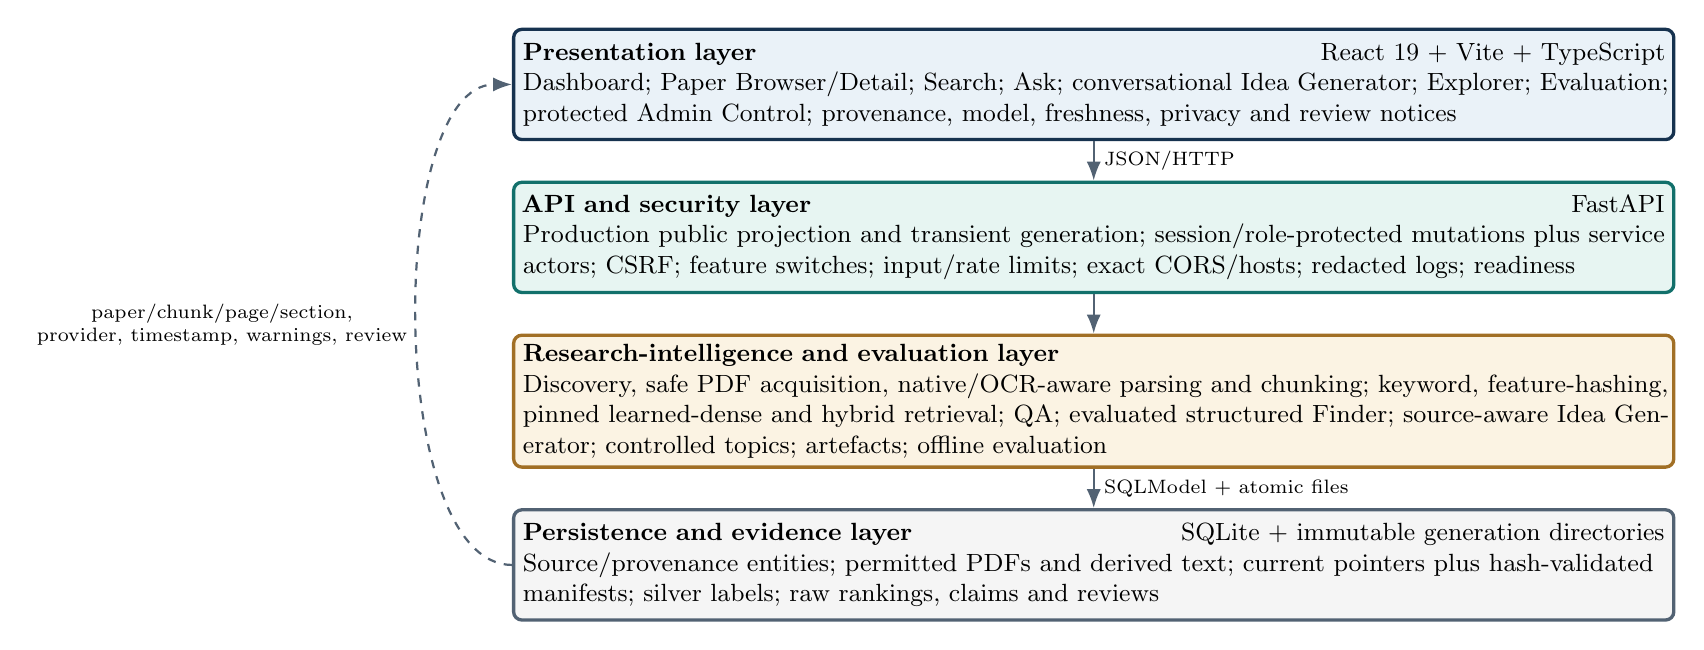
\begin{tikzpicture}[node distance=5mm]
  \node[layerbox] (ui) {\textbf{Presentation layer} \hfill React 19 + Vite + TypeScript\\Dashboard; Paper Browser/Detail; Search; Ask; conversational Idea Generator; Explorer; Evaluation; protected Admin Control; provenance, model, freshness, privacy and review notices};
  \node[layerbox, below=of ui, fill=PaleTeal, draw=Teal!80!black] (api) {\textbf{API and security layer} \hfill FastAPI\\Production public projection and transient generation; session/role-protected mutations plus service actors; CSRF; feature switches; input/rate limits; exact CORS/hosts; redacted logs; readiness};
  \node[layerbox, below=of api, fill=PaleGold, draw=Gold!80!black] (logic) {\textbf{Research-intelligence and evaluation layer}\\Discovery, safe PDF acquisition, native/OCR-aware parsing and chunking; keyword, feature-hashing, pinned learned-dense and hybrid retrieval; QA; evaluated structured Finder; source-aware Idea Generator; controlled topics; artefacts; offline evaluation};
  \node[layerbox, below=of logic, fill=gray!8, draw=Slate] (data) {\textbf{Persistence and evidence layer} \hfill SQLite + immutable generation directories\\Source/provenance entities; permitted PDFs and derived text; current pointers plus hash-validated manifests; silver labels; raw rankings, claims and reviews};
  \draw[arrow] (ui) -- node[right,font=\scriptsize]{JSON/HTTP} (api);
  \draw[arrow] (api) -- (logic);
  \draw[arrow] (logic) -- node[right,font=\scriptsize]{SQLModel + atomic files} (data);
  \draw[dashedarrow] (data.west) .. controls +(-16mm,0) and +(-16mm,0) .. node[left,font=\scriptsize,align=center]{paper/chunk/page/section,\\provider, timestamp, warnings, review} (ui.west);
\end{tikzpicture}
}
\caption[Layered system architecture and provenance return path.]{Layered system architecture. The dashed path represents provenance and review data returned from storage to public evidence displays. Text labels provide the non-color encoding.}
\label{fig:thesis-architecture}
\end{figure}

\section{Design principles}

Seven principles govern the design. First, derived index state is authoritative only when its manifest and active generation pointer match the current corpus. Second, technical eligibility never implies publication or redistribution approval. Third, source facts, paper-informed ideas, and general suggestions use distinct fields and labels. Fourth, AI review has a distinct \texttt{ai\_reviewed} state and cannot create human approval. Fifth, public requests are privacy-minimised and administrative mutations are authenticated. Sixth, model and retrieval identity are recorded at generation time. Seventh, missing dependencies or evidence produce explicit unavailable, stale, partial, \texttt{support\_unverified}, or needs-reprocess states instead of silent success.

\section{Persistence and traceability model}

\Cref{fig:entity-model} summarises the entities. Papers/chunks store extraction, chunk and approved-public generations; outputs retain structured source identifiers. Controlled topics link papers and canonical identities. Each transition appends an actor-typed, request-attributed, hash-linked \texttt{ReviewEvent}, preserving history without treating AI review as human approval.

\begin{figure}[htbp]
\centering
\resizebox{0.97\textwidth}{!}{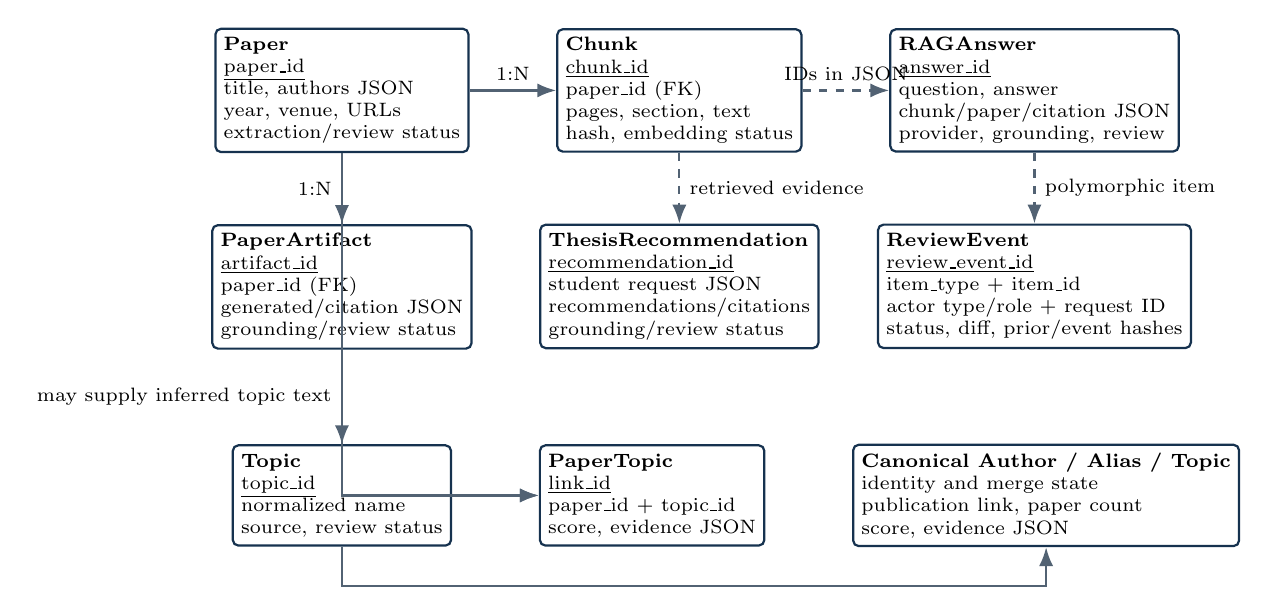
\begin{tikzpicture}[node distance=9mm and 11mm]
  \node[entity] (paper) {\textbf{Paper}\\\underline{paper\_id}\\title, authors JSON\\year, venue, URLs\\extraction/review status};
  \node[entity, right=of paper] (chunk) {\textbf{Chunk}\\\underline{chunk\_id}\\paper\_id (FK)\\pages, section, text\\hash, embedding status};
  \node[entity, right=of chunk] (answer) {\textbf{RAGAnswer}\\\underline{answer\_id}\\question, answer\\chunk/paper/citation JSON\\provider, grounding, review};

  \node[entity, below=of paper] (artifact) {\textbf{PaperArtifact}\\\underline{artifact\_id}\\paper\_id (FK)\\generated/citation JSON\\grounding/review status};
  \node[entity, below=of chunk] (recommendation) {\textbf{ThesisRecommendation}\\\underline{recommendation\_id}\\student request JSON\\recommendations/citations\\grounding/review status};
  \node[entity, below=of answer] (review) {\textbf{ReviewEvent}\\\underline{review\_event\_id}\\item\_type + item\_id\\actor type/role + request ID\\status, diff, prior/event hashes};

  \node[entity, below=12mm of artifact] (topic) {\textbf{Topic}\\\underline{topic\_id}\\normalized name\\source, review status};
  \node[entity, right=of topic] (papertopic) {\textbf{PaperTopic}\\\underline{link\_id}\\paper\_id + topic\_id\\score, evidence JSON};
  \node[entity, right=of papertopic] (authortopic) {\textbf{Canonical Author / Alias / Topic}\\identity and merge state\\publication link, paper count\\score, evidence JSON};

  \draw[arrow] (paper) -- node[above,font=\scriptsize]{1:N} (chunk);
  \draw[dashedarrow] (chunk) -- node[above,font=\scriptsize]{IDs in JSON} (answer);
  \draw[arrow] (paper) -- node[left,font=\scriptsize]{1:N} (artifact);
  \draw[dashedarrow] (chunk) -- node[right,font=\scriptsize]{retrieved evidence} (recommendation);
  \draw[dashedarrow] (answer) -- node[right,font=\scriptsize]{polymorphic item} (review);
  \draw[arrow] (paper) |- (papertopic);
  \draw[arrow] (topic) -- (papertopic);
  % Route below the middle association node.  An explicit waypoint avoids the
  % ambiguous border-intersection route that PGF reports when ``-|'' crosses
  % the PaperTopic node before entering AuthorTopic.
  \draw[arrow] (topic.south) |- ($(papertopic.south)+(0,-5mm)$) -| (authortopic.south);
  \draw[dashedarrow] (artifact) -- node[left,font=\scriptsize]{may supply inferred topic text} (topic);
\end{tikzpicture}
}
\caption[Principal persistence and provenance entities.]{Principal persistence and provenance entities. Solid arrows denote ownership/foreign-key relations; dashed arrows denote evidence or polymorphic references.}
\label{fig:entity-model}
\end{figure}

\section{Authoritative index design}

Each vector manifest binds the corpus and ordered chunks/hashes to provider/model/revision, dimension/normalisation, configuration/code/index hashes, role, and completeness. A rebuild validates an immutable generation, commits matching database status, then atomically moves the current pointer; failure leaves the prior pointer active. Demo indexes cannot target the canonical location, and validators reject missing, partial, stale, or mismatched state.

Feature hashing is a 256-dimensional signed lexical projection, not learned semantics. Dense retrieval pins \texttt{all-MiniLM-L6-v2} revision \texttt{826711e...a1def9}, its artifact hash, 384 dimensions, normalization, CPU/window pooling, and license. Production Ollama use requires an approved model/digest. An explicit local-demo policy may permit installed models while still checking the observed digest before and after generation; absent response attestation is recorded as a mutable-tag limitation.

\section{Security and privacy boundaries}

Public reads/generation are separate from technical evaluation and protected mutations. Production metadata requires human approval, published state and cleared rights; searchable text also requires approved extraction/current public generation. No audited record met the full predicate, so production evidence routes fail closed. Local administrators authenticate with Argon2id passwords and HttpOnly, SameSite sessions; a readable CSRF cookie must match the mutation header. Idle/absolute expiry, lockout, forced temporary-password replacement, role restrictions, production HTTPS/host/CORS checks, size/rate limits, redaction, SSRF/redirect controls, and PDF limits address principal threats. Environment-digested bearer service actors remain available for bounded automation.

Student interests, skills, time, constraints, topic preferences, and Idea Generator conversation turns remain client-side/in-request and are not persisted by default. Public generated-output serializers omit private reviewer notes and draft corrections. This minimisation reduces privacy risk but does not replace an institutional privacy review for a deployed service.

\chapter{Data Collection and Processing}
\label{ch:data}

\section{Catalog and acquisition}

The catalog contains \CatalogPaperCount{} publication records derived from the TTLAB archive and stored in deterministic seed JSON. The discovery/import path normalises titles and URLs, assigns stable identifiers, preserves absent metadata as missing, and records provenance/review state. PDF acquisition uses allowed hosts and public IP resolution, bounded redirects, timeouts, content-length and byte limits, content-type and PDF-signature validation, and explicit failure categories. It does not bypass authentication, paywalls, or access controls.

The frozen audit records \AvailablePdfCount{} available PDFs, \NoPdfUrlCount{} records with no PDF URL, \PdfNetworkErrorCount{} network error, and \PdfNotFoundCount{} not-found result. Of the available documents, \EligiblePaperCount{} matched their catalog identity and entered the experimental corpus; \MismatchPaperCount{} possible PDF/title mismatches were excluded. The remaining \NoTextPaperCount{} catalog records are visible as needs-review/no-text records rather than being silently absent. \Cref{fig:ingestion} shows the full pipeline, and \cref{fig:corpus-status} shows the resulting paper-level eligibility categories.

\begin{figure}[htbp]
\centering
\resizebox{0.99\textwidth}{!}{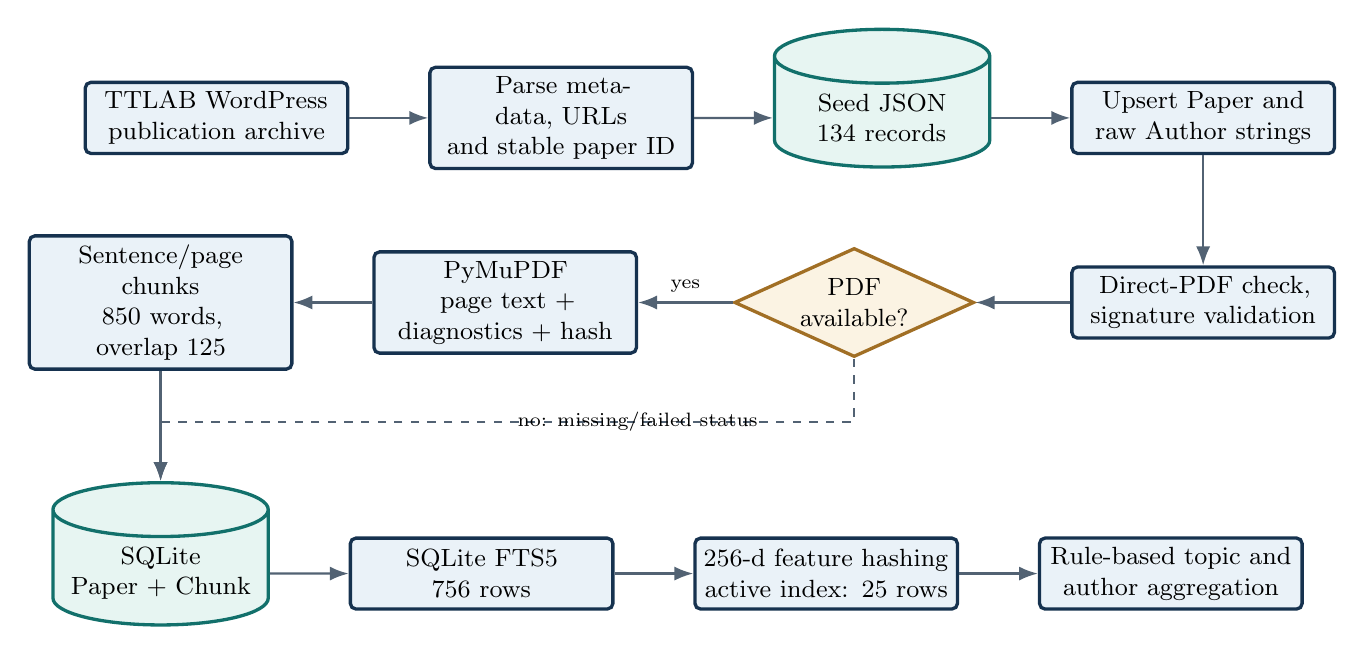
\begin{tikzpicture}[node distance=8mm and 10mm]
  \node[flowbox] (archive) {TTLAB WordPress\\publication archive};
  \node[flowbox, right=of archive] (discover) {Parse metadata, URLs\\and stable paper ID};
  \node[datastore, right=of discover] (seed) {Seed JSON\\134 records};
  \node[flowbox, right=of seed] (import) {Upsert Paper and\\raw Author strings};

  \node[flowbox, below=14mm of import] (download) {Direct-PDF check,\\signature validation};
  \node[decision, left=12mm of download] (available) {PDF\\available?};
  \node[flowbox, left=12mm of available] (extract) {PyMuPDF page text +\\diagnostics + hash};
  \node[flowbox, left=of extract] (chunk) {Sentence/page chunks\\850 words, overlap 125};

  \node[datastore, below=14mm of chunk] (db) {SQLite\\Paper + Chunk};
  \node[flowbox, right=of db] (fts) {SQLite FTS5\\756 rows};
  \node[flowbox, right=of fts] (hash) {256-d feature hashing\\active index: 25 rows};
  \node[flowbox, right=of hash] (topics) {Rule-based topic and\\author aggregation};

  \draw[arrow] (archive) -- (discover);
  \draw[arrow] (discover) -- (seed);
  \draw[arrow] (seed) -- (import);
  \draw[arrow] (import) -- (download);
  \draw[arrow] (download) -- (available);
  \draw[arrow] (available) -- node[above,font=\scriptsize]{yes} (extract);
  \draw[arrow] (extract) -- (chunk);
  \draw[arrow] (chunk) -- (db);
  \draw[arrow] (db) -- (fts);
  \draw[arrow] (fts) -- (hash);
  \draw[arrow] (hash) -- (topics);
  \draw[dashedarrow] (available.south) -- ++(0,-8mm) -| node[pos=0.25,right,font=\scriptsize]{no: missing/failed status} (db.north);
\end{tikzpicture}
}
\caption[Deterministic ingestion and authoritative indexing pipeline.]{Deterministic ingestion and authoritative indexing pipeline. The optional OCR stage records status/provenance but was not used in the frozen corpus.}
\label{fig:ingestion}
\end{figure}

\begin{figure}[htbp]
\centering
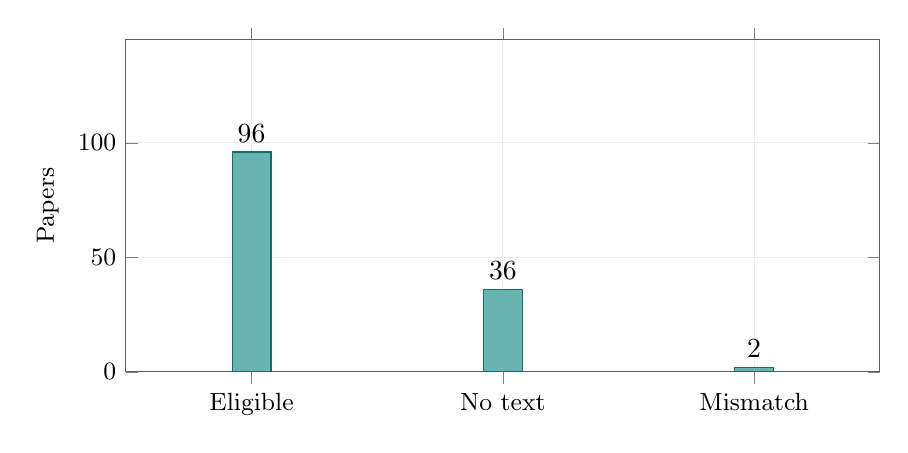
\begin{tikzpicture}
\begin{axis}[
  ybar,
  width=0.92\linewidth,
  height=58mm,
  ymin=0,
  ymax=145,
  bar width=14pt,
  symbolic x coords={Eligible,No text,Mismatch},
  xtick=data,
  ylabel={Papers},
  nodes near coords,
  nodes near coords align={vertical},
  axis line style={draw=Slate},
  tick label style={font=\small},
  label style={font=\small},
  enlarge x limits=0.25,
  grid=major,
  grid style={gray!15}
]
\addplot[fill=Teal!65,draw=Teal!80!black] coordinates {(Eligible,96) (No text,36) (Mismatch,2)};
\end{axis}
\end{tikzpicture}

\caption[Frozen catalog eligibility.]{Frozen catalog eligibility: \EligiblePaperCount{} eligible full-text papers, \NoTextPaperCount{} records without eligible text, and \MismatchPaperCount{} PDF/title mismatch exclusions. These are inventory counts, not quality scores.}
\label{fig:corpus-status}
\end{figure}

\section{Extraction and OCR-aware diagnostics}

PyMuPDF extracts native text page by page and records page/character/word counts, empty pages, extraction status, and hashes. Content classification distinguishes textual, mixed, and unknown records. The repaired pipeline detects low-text/image-heavy pages and supports optional OCR with page-level engine/configuration, confidence/status, and review flags. OCR dependencies are optional and fail explicitly. All \CatalogPaperCount{} records in the frozen snapshot have \texttt{ocr\_status=not\_requested}; therefore, the thesis reports no OCR accuracy or latency.

The \AvailablePdfCount{} extracted PDFs contain \ExtractedPageCount{} pages and \ExtractedWordCount{} native-extraction words. These totals describe the local source snapshot; they are not included in the sanitized release. The suspected identity mismatches account for \MismatchChunkCount{} excluded chunks. The raw chunk table contains \RawChunkCount{} rows, while the eligible experiment and authoritative indexes contain \EligibleChunkCount{} rows.

\section{Page-aware chunking and sections}

Extracted sentences retain their page number. Chunks target 850 words with a 5,000-character limit and 125-word overlap; identifiers incorporate paper, sequence, page span, and source hash. Section names are inferred from headings and layout cues, with \texttt{Unknown} preserved when evidence is insufficient. Among eligible chunks, \EligibleUnknownChunkCount{} are unknown-section chunks (\EligibleUnknownChunkPercent\%).

A \SectionSilverCaseCount{}-case stratified AI-reviewed silver sample compared current section labels with source passages. Exact accuracy was \SectionSilverAccuracy{}, labeled coverage 0.900, macro precision \SectionSilverMacroPrecision{}, and macro recall \SectionSilverMacroRecall{}. Seven creation decisions required revision. These results support using section labels as a reranking feature with caution, not as authoritative document structure.

\section{Metadata and author identity}

The malformed \texttt{Click to View} author parser artifact was removed by an idempotent migration. The schema now stores canonical author rows, aliases, identity/merge state, and review status. The audit found \RawAuthorRowCount{} author rows: \CanonicalAuthorCount{} unresolved active canonical identities, two merged rows, and one invalid row. Exact alias collisions, eligible authorship mismatches, excluded-paper leakage, and prohibited expertise overclaims were all zero in the executed audit. \PossibleAuthorMergeCount{} possible initial/full-name or spelling pairs remain deliberately unmerged pending authoritative confirmation.

DOI, abstract, keyword, venue, and date fields carry provenance and review fields. Unverified metadata remain empty. Author-topic links are derived only from eligible indexed publication authorship and paper topics; their UI wording explicitly disclaims availability, endorsement, supervision, or expertise beyond this corpus.

\section{Corpus distribution and release boundary}

\begin{figure}[htbp]
\centering
\begin{tikzpicture}
\begin{axis}[
  ybar,
  width=0.97\linewidth,
  height=65mm,
  ymin=0,
  bar width=7pt,
  xlabel={Publication year in seed metadata},
  ylabel={Papers},
  xtick=data,
  x tick label style={rotate=45,anchor=east,font=\scriptsize},
  y tick label style={font=\small},
  label style={font=\small},
  grid=major,
  grid style={gray!15},
  nodes near coords,
  nodes near coords style={font=\tiny}
]
\addplot[fill=Navy!65,draw=Navy] table[x=year,y=count,col sep=comma] {generated/year_distribution.csv};
\end{axis}
\end{tikzpicture}

\caption[Publication-year distribution in catalog metadata.]{Publication-year distribution in the catalog metadata. Missing or uncertain years remain represented in the generated source data rather than being imputed.}
\label{fig:years}
\end{figure}

The year distribution in \cref{fig:years} characterises the seed, not full-text eligibility. Raw PDFs, extracted text, chunks, local database, and indexes are excluded from the sanitized release because TTLAB project authorization does not itself confer redistribution rights for every third-party paper. The release retains redistributable metadata, schemas, prompts without restricted passages, labels, aggregate/raw sanitized results, source hashes, and reacquisition instructions.

\chapter{Implementation}
\label{ch:implementation}

\section{Technology stack and interface}

The backend uses Python, FastAPI, SQLModel, Pydantic settings, SQLite, and PyMuPDF. The frontend uses React, TypeScript, and Vite. Eight views expose dashboard statistics, papers, search, Ask TTLAB, extension recommendations, topic/author exploration, administrative review, and evaluation. \Cref{fig:dashboard-shot,fig:search-shot} show the audited runtime.

\begin{figure}[htbp]
\centering
\projectScreenshot{figures/screenshots/dashboard.png}{0.96\textwidth}
\caption{Dashboard in the audited browser session. The empty top-topic widget contrasts with populated explorer data and is retained as failure evidence.}
\label{fig:dashboard-shot}
\end{figure}

\begin{figure}[htbp]
\centering
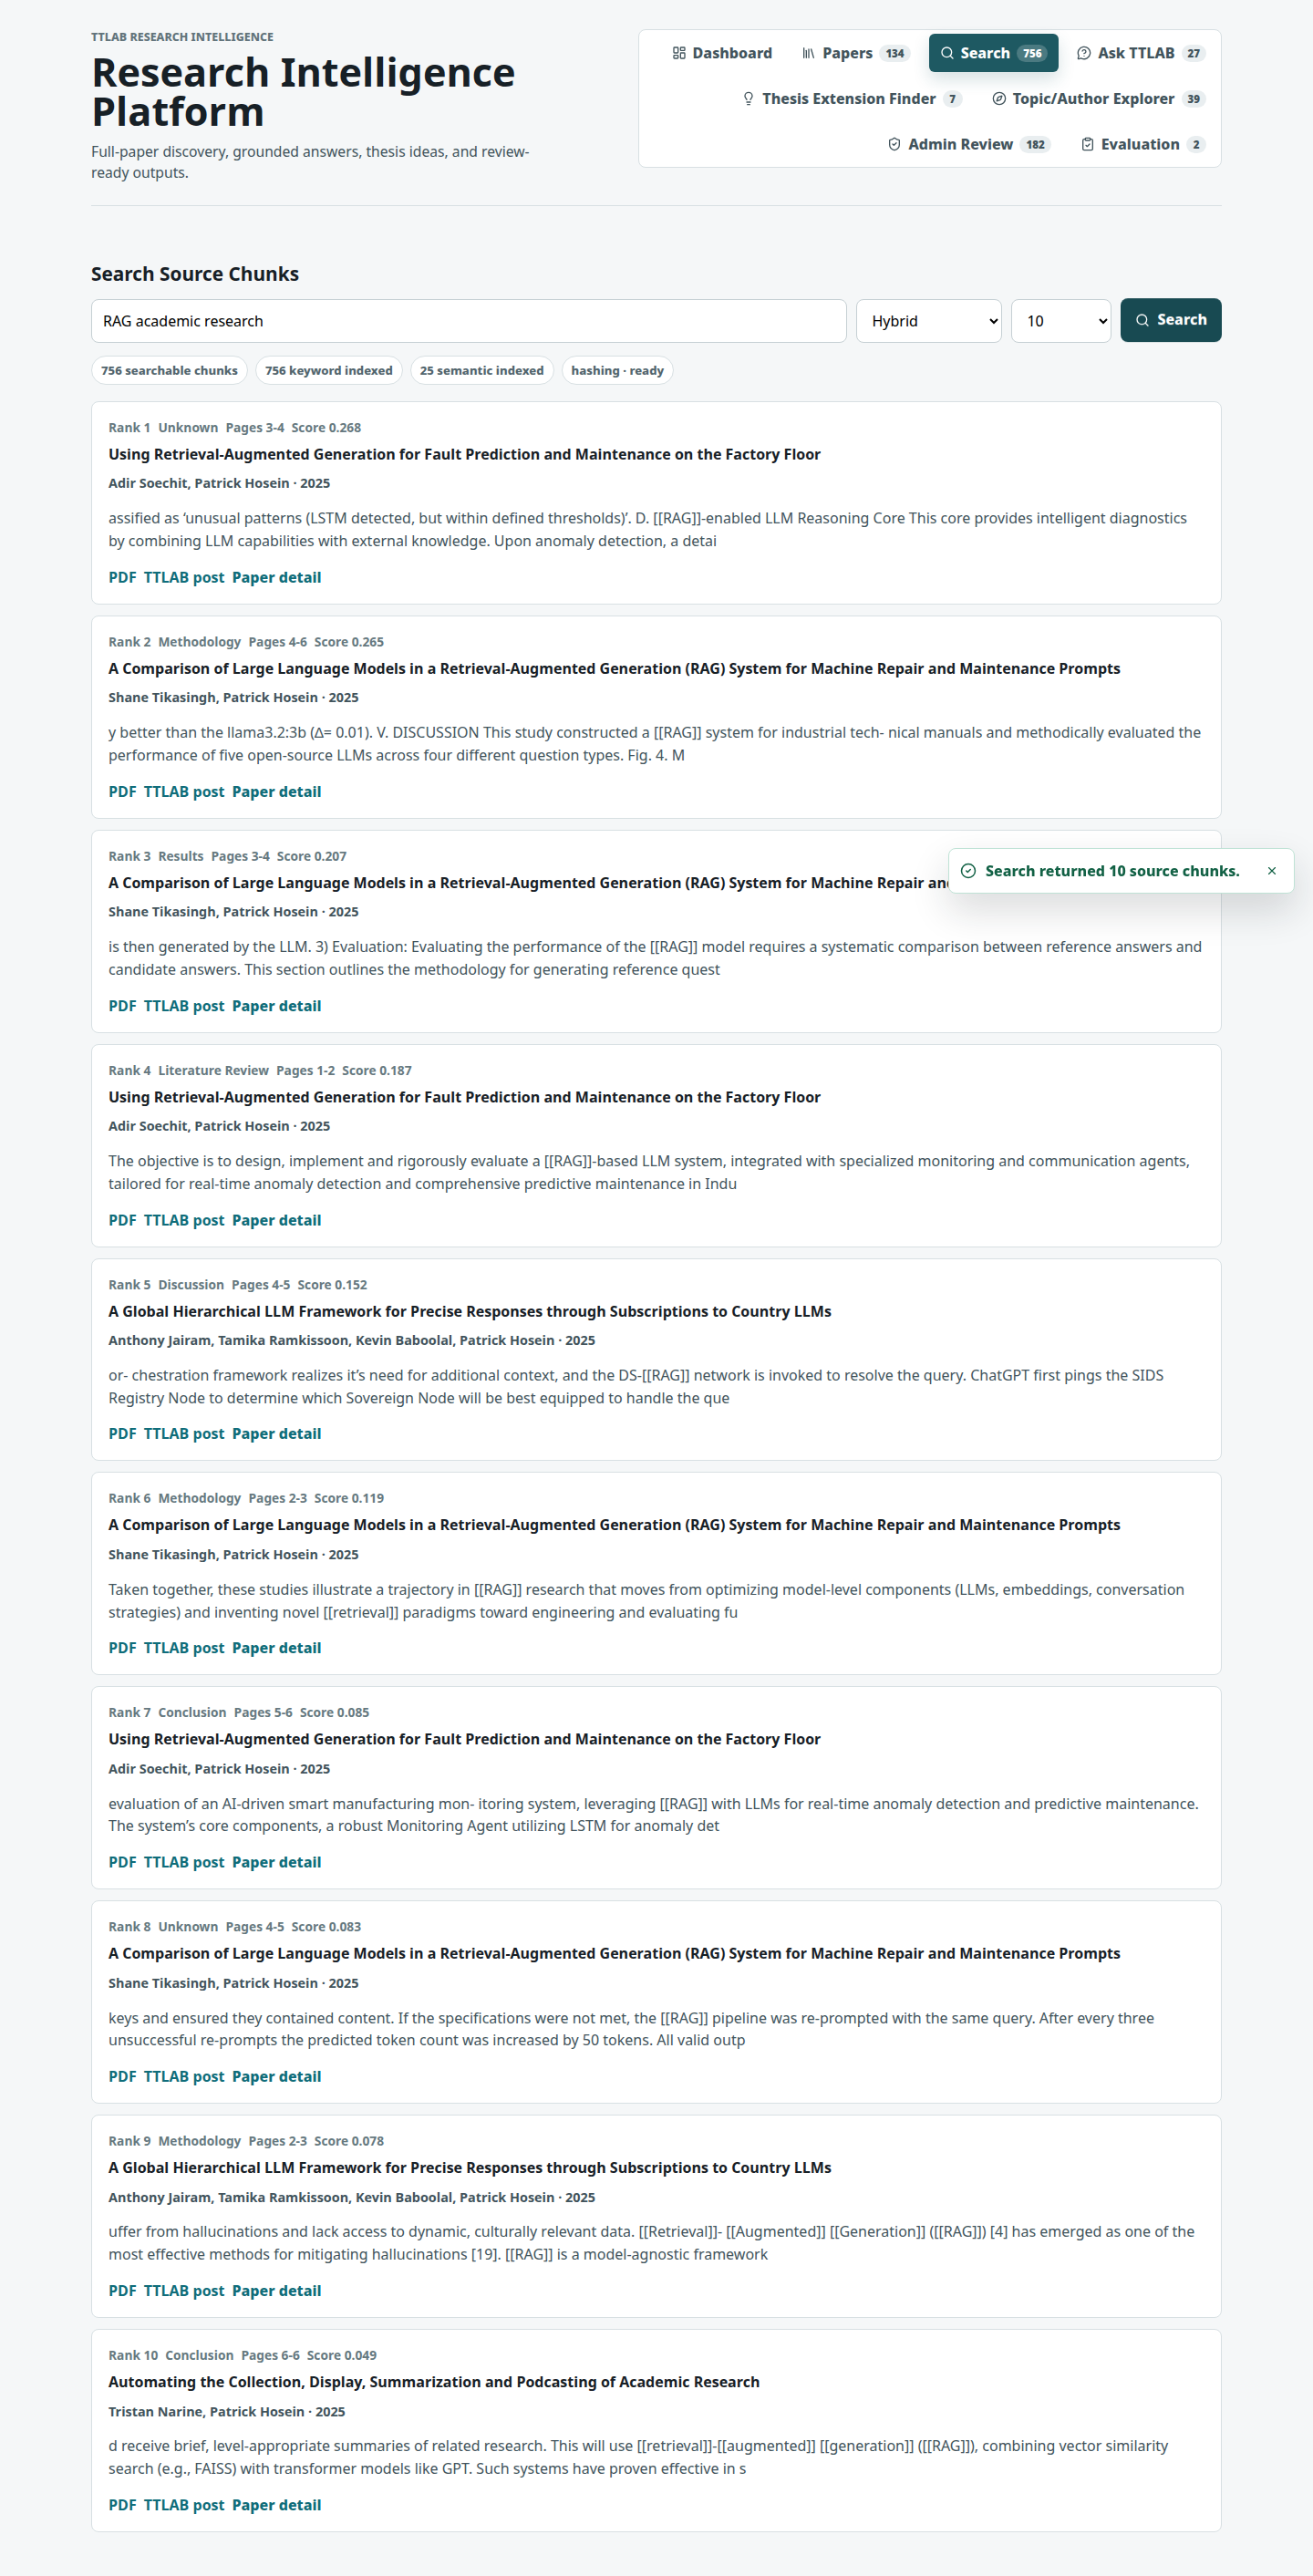
\includegraphics[width=0.96\textwidth,trim=0 950bp 0 0,clip]{figures/screenshots/search-results.png}
\caption{Search results with mode, scores, paper metadata, pages, and source snippets. The full-page capture is deliberately cropped to its top results for legibility.}
\label{fig:search-shot}
\end{figure}

Navigation is held in React state rather than URL routes, so refreshing returns to the dashboard and views are not deep-linkable.

\section{Keyword and hashing-vector retrieval}

SQLite FTS5 indexes all chunk text and returns its \texttt{bm25()} rank, transformed by
\begin{equation}
K = \frac{1}{1+|r_{\mathrm{FTS}}|}.
\label{eq:fts-transform}
\end{equation}
A deterministic fallback combines term frequency and query coverage when FTS is unavailable.

The vector path maps token $t$ into one of $d=256$ coordinates and a sign using SHA-256. For document $x$, the unnormalised coordinate is
\begin{equation}
z_j(x)=\sum_{t\in x}\mathbb{I}[h(t)=j]s(t), \qquad
\mathbf{v}(x)=\frac{\mathbf{z}(x)}{\lVert\mathbf{z}(x)\rVert_2}.
\label{eq:hashing}
\end{equation}
Similarity is the dot product $V=\mathbf{v}(q)^\top\mathbf{v}(c)$, equivalent to cosine similarity after normalisation. This is feature hashing \cite{weinberger2009featurehashing}, not a learned semantic encoder.

\section{Hybrid scoring and diversification}

Current working-tree code removes a fixed stop-word set, applies fixed domain query expansions, and computes
\begin{equation}
H=\operatorname{clip}_{[0,1]}(0.42K+0.48V+M+S+E+T),
\label{eq:hybrid}
\end{equation}
where $M$ is metadata match, $S$ an intent-dependent section boost, $E$ an evidence-quality adjustment, and $T$ topical alignment. A greedy penalty reduces repeated or adjacent chunks from the same paper. The coefficients are hand-authored; no tuning or ablation evidence exists.

\section{Question answering}

The workflow in \cref{fig:rag-workflow} retrieves chunks, composes an answer with a deterministic offline provider or local Ollama, attaches citations, verifies structural properties, persists the result, and displays the answer with source pages and warnings.

\begin{figure}[htbp]
\centering
\begingroup\hfuzz=100pt\resizebox{\textwidth}{!}{\begingroup\hfuzz=100pt
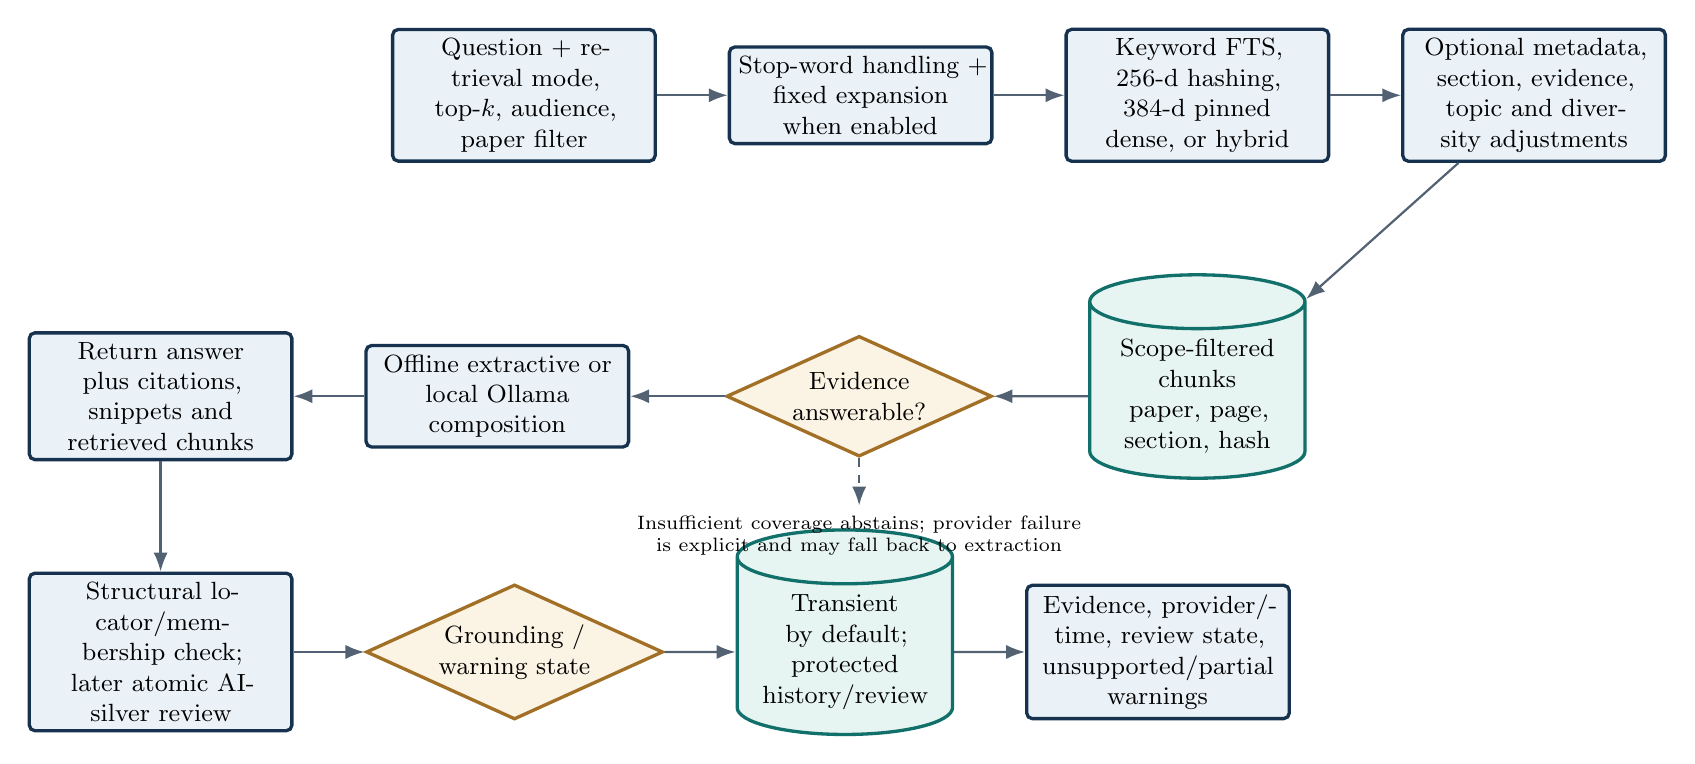
\begin{tikzpicture}[node distance=8mm and 9mm]
  \node[flowbox] (question) {Question + retrieval mode,\\top-$k$, audience, paper filter};
  \node[flowbox, right=of question] (prepare) {Stop-word handling +\\fixed expansion when enabled};
  \node[flowbox, right=of prepare] (retrieve) {Keyword FTS, 256-d hashing,\\384-d pinned dense, or hybrid};
  \node[flowbox, right=of retrieve] (rerank) {Optional metadata, section, evidence,\\topic and diversity adjustments};

  \node[datastore, below=14mm of retrieve] (chunks) {Scope-filtered chunks\\paper, page, section, hash};
  \node[decision, left=12mm of chunks] (provider) {Evidence\\answerable?};
  \node[flowbox, left=12mm of provider] (compose) {Offline extractive or\\local Ollama composition};
  \node[flowbox, left=of compose] (cite) {Return answer plus citations,\\snippets and retrieved chunks};

  \node[flowbox, below=14mm of cite] (verify) {Structural locator/membership check;\\later atomic AI-silver review};
  \node[decision, right=of verify] (status) {Grounding /\\warning state};
  \node[datastore, right=of status] (persist) {Transient by default;\\protected history/review};
  \node[flowbox, right=of persist] (display) {Evidence, provider/time, review state,\\unsupported/partial warnings};

  \draw[arrow] (question) -- (prepare);
  \draw[arrow] (prepare) -- (retrieve);
  \draw[arrow] (retrieve) -- (rerank);
  \draw[arrow] (rerank) -- (chunks);
  \draw[arrow] (chunks) -- (provider);
  \draw[arrow] (provider) -- (compose);
  \draw[arrow] (compose) -- (cite);
  \draw[arrow] (cite) -- (verify);
  \draw[arrow] (verify) -- (status);
  \draw[arrow] (status) -- (persist);
  \draw[arrow] (persist) -- (display);
  \draw[dashedarrow] (provider.south) -- ++(0,-6mm) node[below,font=\scriptsize,align=center]{Insufficient coverage abstains; provider failure\\is explicit and may fall back to extraction};
\end{tikzpicture}
\endgroup
}\endgroup
\caption{Implemented search and RAG workflow. The verifier checks structure, membership, and lexical overlap rather than semantic entailment.}
\label{fig:rag-workflow}
\end{figure}

The Ollama adapter uses a low-temperature, source-restricted prompt and falls back on error. The OpenAI provider branch raises a not-implemented error. The verifier requires retrieved chunks, complete citation fields, citation membership, and at least 0.08 answer-to-snippet token overlap. Therefore, its \texttt{grounded} label means structurally/lexically grounded only.

\begin{figure}[htbp]
\centering
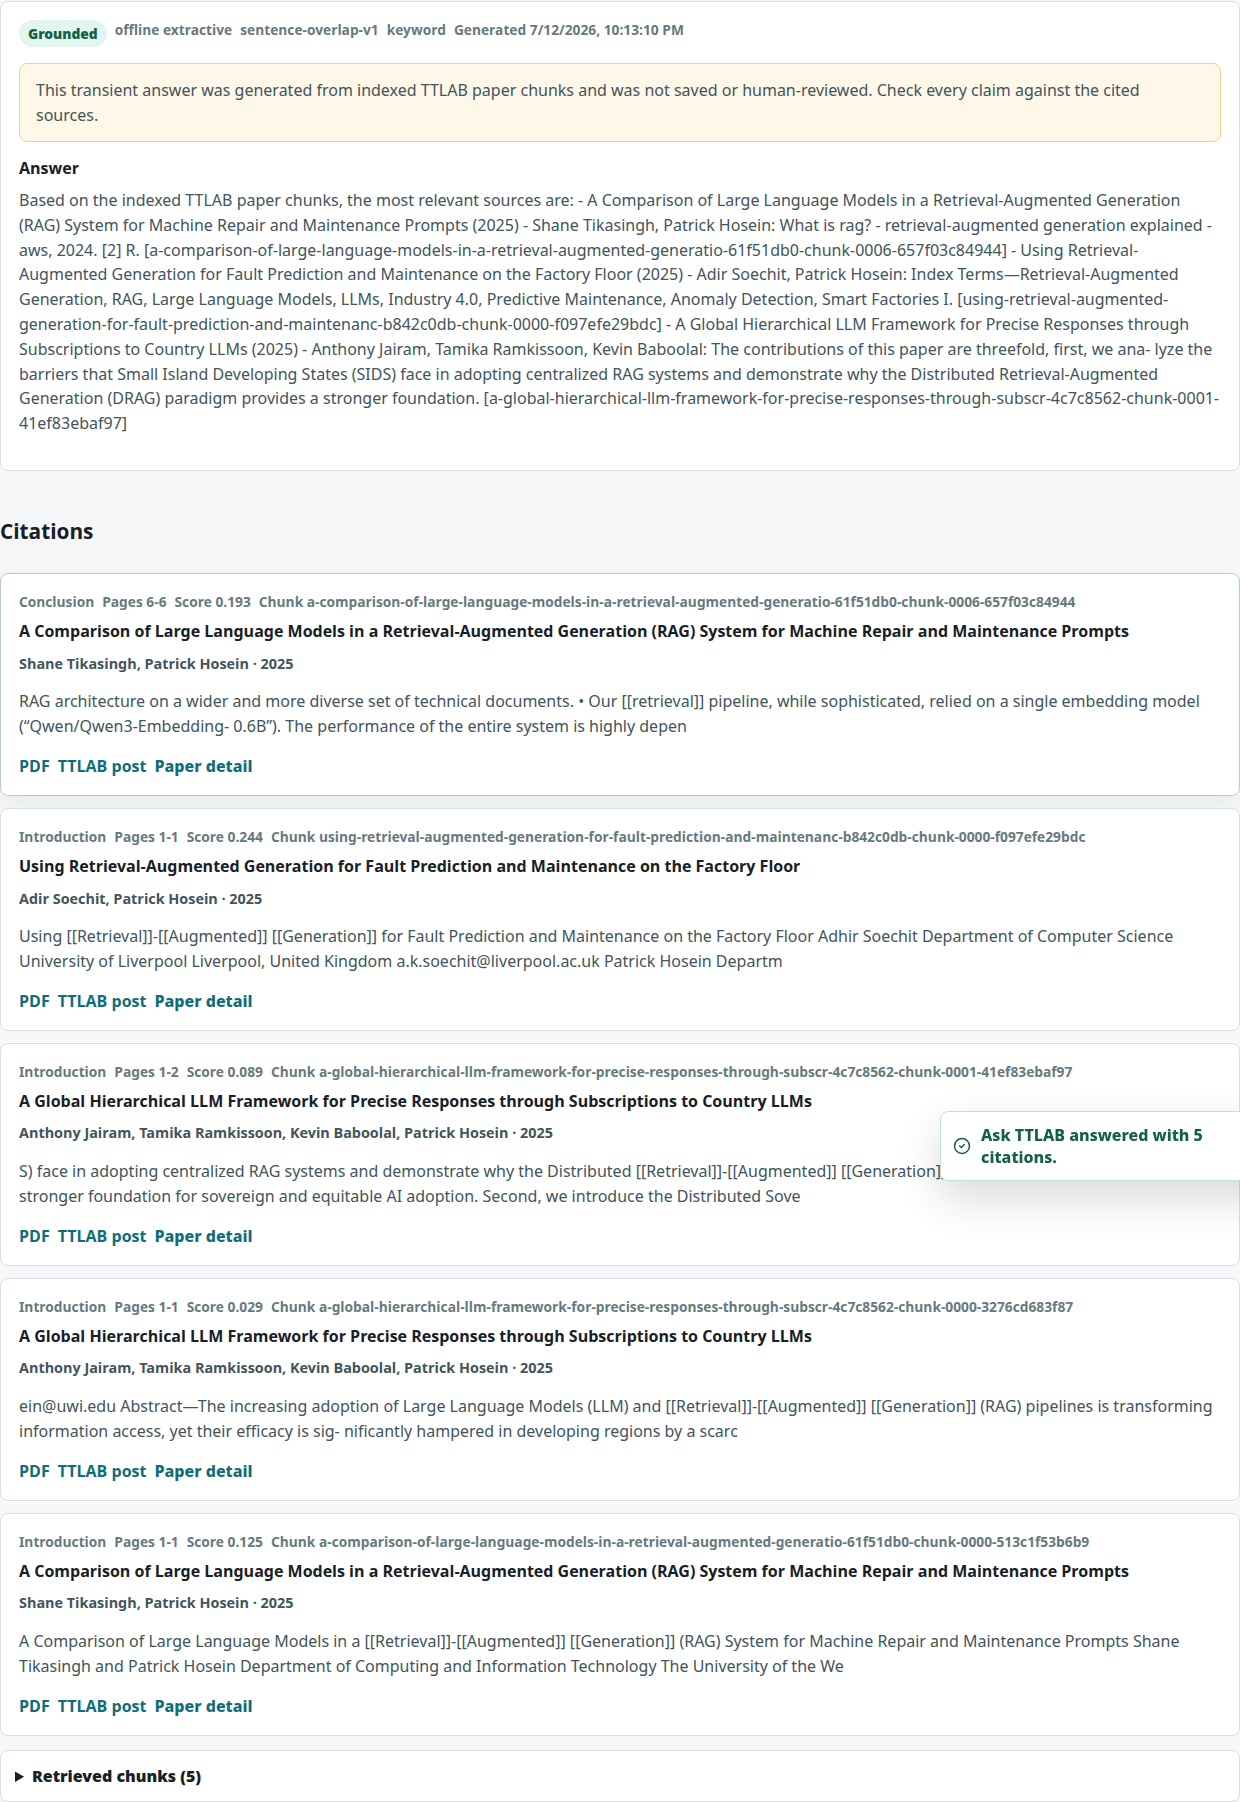
\includegraphics[width=0.96\textwidth,trim=0 900bp 0 0,clip]{figures/screenshots/ask-answer.png}
\caption{Ask TTLAB response showing generated-answer notice, grounding state, and cited papers. The full-page capture is deliberately cropped to the answer and leading citations.}
\label{fig:ask-shot}
\end{figure}

\section{Thesis-extension recommendations}

\Cref{fig:recommendation-workflow} shows the deterministic workflow. Candidate paper score $R$ is
\begin{align}
R={}&0.30r+0.20i+0.15s+0.10d+0.10t \\
   &+0.10f+0.05e-0.20a,
\label{eq:recommendation}
\end{align}
where the terms represent retrieval relevance, interest, skill, data, time, difficulty fit, evidence strength, and avoided-topic match. The output distinguishes an explicit, inferred, or absent source gap from the system's suggested extension.

\begin{figure}[htbp]
\centering
\begingroup\hfuzz=100pt\resizebox{\textwidth}{!}{\begingroup\hfuzz=100pt
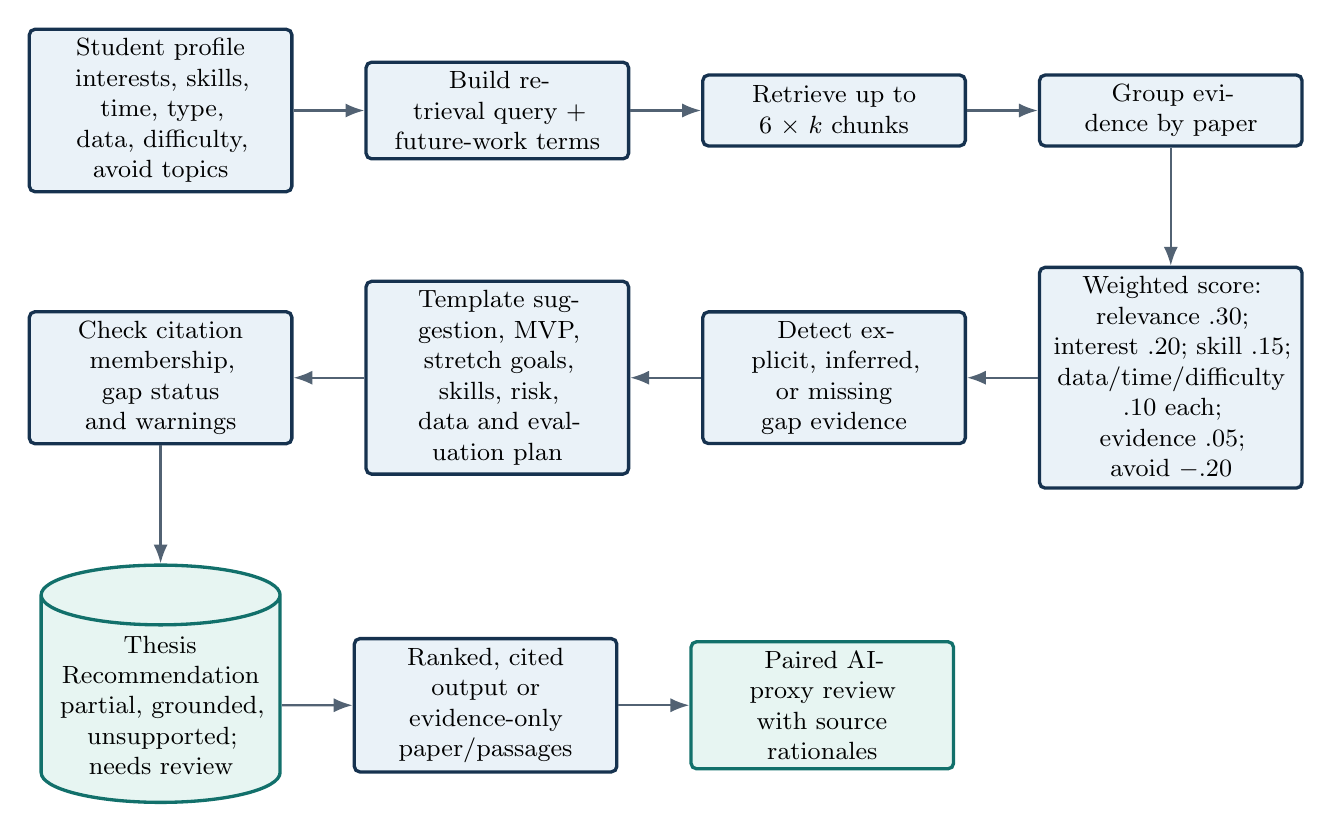
\begin{tikzpicture}[node distance=8mm and 9mm]
  \node[flowbox] (profile) {Student profile\\interests, skills, time, type,\\data, difficulty, avoid topics};
  \node[flowbox, right=of profile] (query) {Build retrieval query +\\future-work terms};
  \node[flowbox, right=of query] (retrieve) {Retrieve up to\\$6\times k$ chunks};
  \node[flowbox, right=of retrieve] (group) {Group evidence by paper};

  \node[flowbox, below=15mm of group] (score) {Weighted score: relevance .30;\\interest .20; skill .15;\\data/time/difficulty .10 each;\\evidence .05; avoid $-.20$};
  \node[flowbox, left=of score] (gap) {Detect explicit, inferred,\\or missing gap evidence};
  \node[flowbox, left=of gap] (draft) {Template suggestion, MVP,\\stretch goals, skills, risk,\\data and evaluation plan};
  \node[flowbox, left=of draft] (verify) {Check citation membership,\\gap status and warnings};

  \node[datastore, text width=28mm, below=15mm of verify] (persist) {Thesis\\Recommendation\\partial, grounded,\\unsupported; needs review};
  \node[flowbox, right=of persist] (ui) {Ranked, cited output or\\evidence-only paper/passages};
  \node[flowbox, right=of ui, fill=PaleTeal, draw=Teal!80!black] (proxy) {Paired AI-proxy review\\with source rationales};

  \draw[arrow] (profile) -- (query);
  \draw[arrow] (query) -- (retrieve);
  \draw[arrow] (retrieve) -- (group);
  \draw[arrow] (group) -- (score);
  \draw[arrow] (score) -- (gap);
  \draw[arrow] (gap) -- (draft);
  \draw[arrow] (draft) -- (verify);
  \draw[arrow] (verify) -- (persist);
  \draw[arrow] (persist) -- (ui);
  \draw[arrow] (ui) -- (proxy);
\end{tikzpicture}
\endgroup
}\endgroup
\caption{Implemented recommendation pipeline and the human-validation stage that has not yet been executed.}
\label{fig:recommendation-workflow}
\end{figure}

\begin{figure}[htbp]
\centering
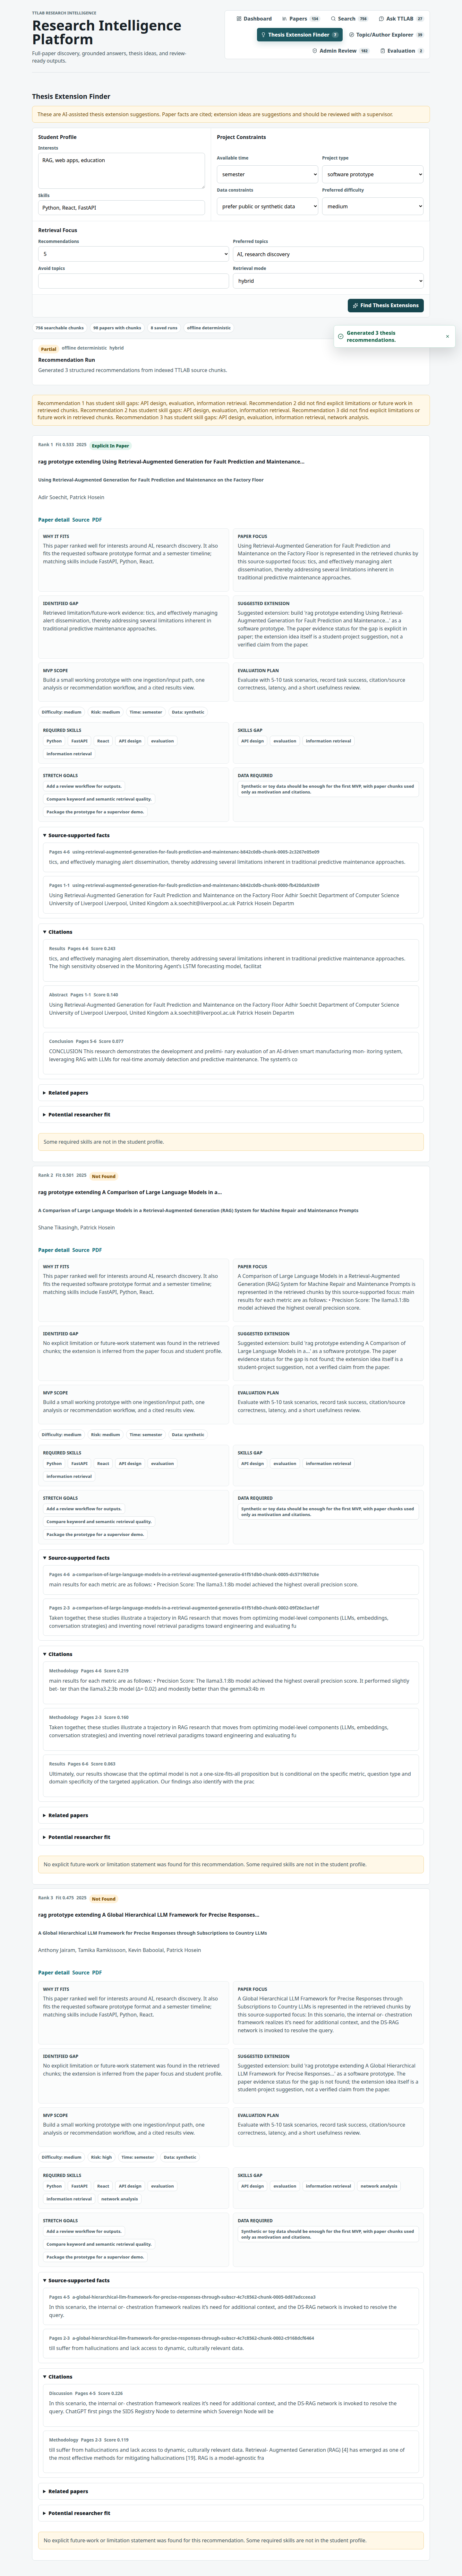
\includegraphics[width=0.96\textwidth,trim=0 6500bp 0 0,clip]{figures/screenshots/extension-results.png}
\caption{Extension Finder profile and leading ranked result with source/gap status. The full-page capture is deliberately cropped before additional result detail.}
\label{fig:extension-shot}
\end{figure}

\section{Topic, author, artefact, and review functions}

Topic discovery uses a fixed 39-topic lexical taxonomy and weighted text sources. It can retain up to eight topic links per paper; author-topic scores aggregate paper topics. Related-paper scoring combines topics, authors, venue, year, lexical overlap, and hashing-vector signals. This is rule-based classification, not topic modelling.

The paper-intelligence generator uses section and lexical priorities to create public and technical summaries, contributions, methods, limitations, future work, suggestions, skills, evaluation ideas, and text-only podcast dialogue. It labels limitations/future work as explicit, inferred, or not found and labels extensions as system suggestions.

Review endpoints can update metadata and statuses and write a review event. The UI exposes queues and status controls, but there is no authentication; the reviewer identity is fixed to \texttt{local\_admin}. \Cref{fig:explorer-shot,fig:admin-shot} show both the explorer's visible identity defect and the review mechanism.

\begin{figure}[htbp]
\centering
\begin{subfigure}{0.49\textwidth}
\projectScreenshot{figures/screenshots/explorer.png}{\linewidth}
\caption{Topic/author explorer.}
\label{fig:explorer-shot}
\end{subfigure}\hfill
\begin{subfigure}{0.49\textwidth}
\projectScreenshot{figures/screenshots/admin-review.png}{\linewidth}
\caption{Administrative review queue.}
\label{fig:admin-shot}
\end{subfigure}
\caption{Discovery and review interfaces. The explorer screenshot retains the ``Click to View'' author artefact.}
\end{figure}

\chapter{Experimental Design}
\label{ch:experiments}

\section{Completed technical verification}

Completed verification comprises source/schema audit, file and database consistency checks, automated tests against an isolated database, representative API probes against a disposable database copy, a clean frontend dependency/build run, browser inspection of eight main surfaces, and LaTeX build/render inspection. These procedures answer whether the snapshot is internally reproducible and demonstrable; they do not answer whether users receive relevant or faithful advice.

\section{Implemented retrieval metrics}

For query $q$, with retrieved paper list $L_q$ and gold set $G_q$, the code reports a binary hit indicator called Recall@$k$:
\begin{equation}
\operatorname{Hit@}k(q)=\mathbb{I}\!\left[G_q\cap L_q[1{:}k]\neq\varnothing\right].
\label{eq:hitk}
\end{equation}
The implementation averages this indicator over queries. It is therefore a hit rate, not set recall $|G_q\cap L_q[1{:}k]|/|G_q|$. Mean reciprocal rank is
\begin{equation}
\operatorname{MRR}=\frac{1}{|Q|}\sum_{q\in Q}\frac{1}{\operatorname{rank}_q},
\label{eq:mrr}
\end{equation}
with zero when no gold paper is retrieved. The sample retrieval and QA files contain empty gold labels and intentionally fail validation, so neither metric has a current result.

\section{Proposed retrieval experiment}

A versioned test set should stratify questions by exact fact, method, result, limitation/future work, topic, author, comparison, and broad intent. Keyword, hashing-vector, and hybrid modes should use the same corpus, cut-offs, and paper filtering. Primary outcomes should include set Recall@3/5, hit rate, MRR, nDCG where graded judgments are available, and per-intent error analysis. Query-expansion and reranking terms should be ablated. The active vector index must first be rebuilt for all 756 chunks and status consistency verified.

\section{Proposed QA evaluation}

Each answer should be decomposed into checkable claims. Reviewers should label whether each claim is entailed by its cited snippet, whether the citation points to the right paper/page, whether important answer points are covered, and whether unsupported general knowledge appears. Automatic RAG measures may supplement but not replace these labels \cite{es2024ragas,saadfalcon2024ares,min2023factscore}. Provider, model hash/tag, prompt, temperature, retrieval list, and fallback state must be stored.

\section{Proposed recommendation evaluation}

Students and supervisors should independently rate paper relevance, gap fidelity, novelty, feasibility for the stated time/skills/data, usefulness of the MVP, risk calibration, and appropriateness of the evaluation plan. Reviewers must separately judge source claims and system suggestions. A comparison baseline could present retrieved papers without generated extension advice. \authorinput{approve participant groups, sample size, rating scales, compensation, consent, and analysis}.

\section{Proposed topic/author and summary evaluation}

Topic evaluation should measure label precision/coverage and reviewer agreement against the fixed taxonomy, including multi-label cases and an ``other'' outcome. Author evaluation should first resolve identities, then assess expertise links. Public and technical summaries should be reviewed for correctness, relevance, coherence, and readability, drawing on human-centred evaluation lessons from SummEval \cite{fabbri2021summeval}.

\section{Evaluation workflow and current state}

\begin{figure}[htbp]
\centering
\begingroup\hfuzz=100pt\resizebox{\textwidth}{!}{\begingroup\hfuzz=100pt
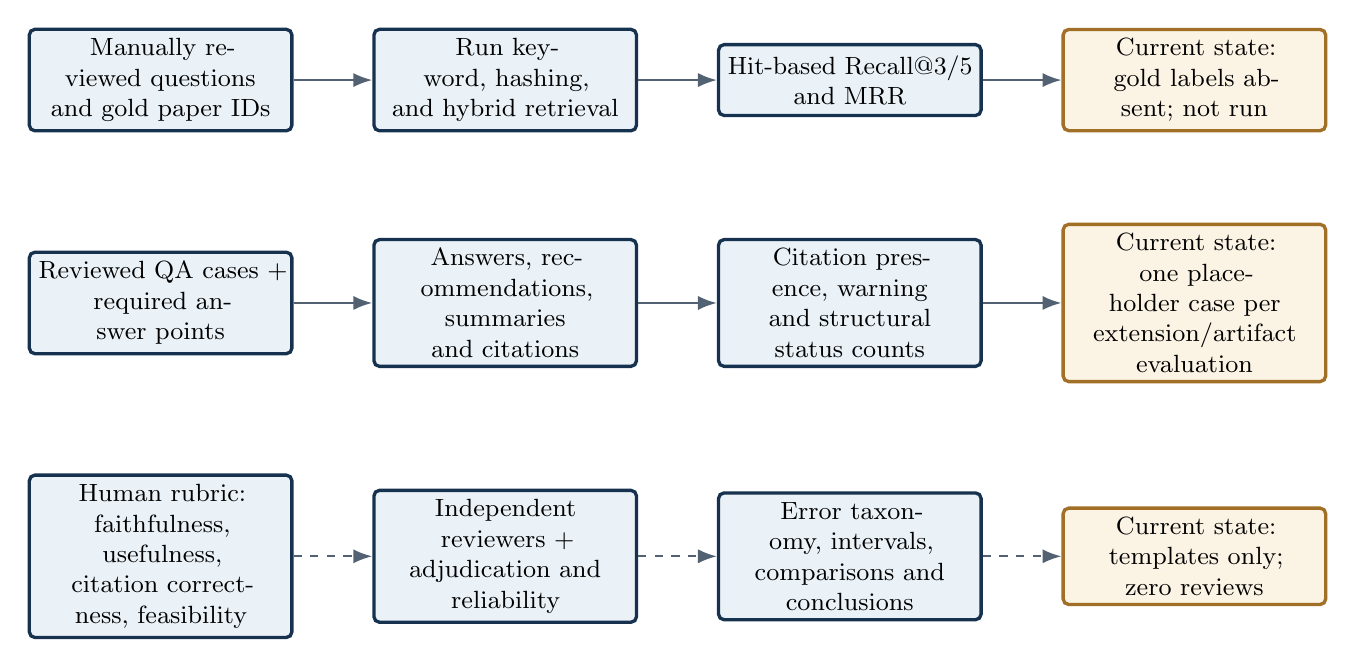
\begin{tikzpicture}[node distance=8mm and 10mm]
  \node[flowbox] (questions) {Manually reviewed questions\\and gold paper IDs};
  \node[flowbox, right=of questions] (retrieval) {Run keyword, hashing,\\and hybrid retrieval};
  \node[flowbox, right=of retrieval] (metrics) {Hit-based Recall@3/5\\and MRR};
  \node[flowbox, right=of metrics, fill=PaleGold, draw=Gold!80!black] (missing) {Current state:\\gold labels absent; not run};

  \node[flowbox, below=15mm of questions] (qa) {Reviewed QA cases +\\required answer points};
  \node[flowbox, right=of qa] (outputs) {Answers, recommendations,\\summaries and citations};
  \node[flowbox, right=of outputs] (automatic) {Citation presence, warning\\and structural status counts};
  \node[flowbox, right=of automatic, fill=PaleGold, draw=Gold!80!black] (placeholder) {Current state:\\one placeholder case per\\extension/artifact evaluation};

  \node[flowbox, below=15mm of qa] (rubric) {Human rubric:\\faithfulness, usefulness,\\citation correctness, feasibility};
  \node[flowbox, right=of rubric] (review) {Independent reviewers +\\adjudication and\\reliability};
  \node[flowbox, right=of review] (analysis) {Error taxonomy, intervals,\\comparisons and conclusions};
  \node[flowbox, right=of analysis, fill=PaleGold, draw=Gold!80!black] (notdone) {Current state:\\templates only; zero reviews};

  \draw[arrow] (questions) -- (retrieval);
  \draw[arrow] (retrieval) -- (metrics);
  \draw[arrow] (metrics) -- (missing);
  \draw[arrow] (qa) -- (outputs);
  \draw[arrow] (outputs) -- (automatic);
  \draw[arrow] (automatic) -- (placeholder);
  \draw[dashedarrow] (rubric) -- (review);
  \draw[dashedarrow] (review) -- (analysis);
  \draw[dashedarrow] (analysis) -- (notdone);
\end{tikzpicture}
\endgroup
}\endgroup
\caption{Implemented and proposed evaluation workflow. Gold retrieval/QA labels and human reviews are absent in the audited snapshot.}
\label{fig:evaluation-workflow}
\end{figure}

\begin{figure}[htbp]
\centering
\projectScreenshot{figures/screenshots/evaluation.png}{0.96\textwidth}
\caption{Evaluation dashboard correctly displaying not-run and placeholder states rather than inferred performance.}
\label{fig:evaluation-shot}
\end{figure}

\chapter{Results}
\label{ch:results}

\section{Corpus and ingestion results (RQ1)}

The pipeline represents all 134 seed records in SQLite and has extracted 98 PDFs into 698 pages and 756 chunks. Thirty-five papers lack PDFs and one is marked download failed (\cref{fig:corpus-status}). PDF, extracted JSON/text, and chunk-file paths are one-to-one for the 98 extracted papers. SQLite integrity checks pass. The observed coverage is therefore 98/134 papers (73.13\%), with the remaining 26.87\% unavailable to full-text retrieval. There is no OCR fallback, and section inference leaves 32.94\% of chunks unknown.

\section{Retrieval and answer traceability (RQ2)}

Keyword FTS contains all 756 chunks. By contrast, the active hashing-vector JSON index contains 25 chunks from three papers (3.31\% of chunks), while 300 SQLite rows retain an indexed-hashing status. \Cref{fig:index-coverage} visualizes this discrepancy.

\begin{figure}[htbp]
\centering
\begingroup\hfuzz=100pt\resizebox{0.90\textwidth}{!}{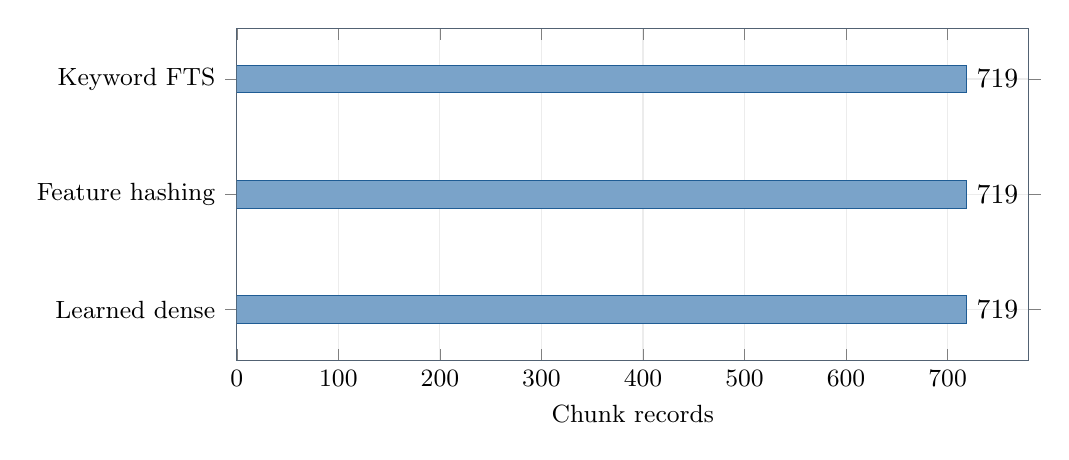
\begin{tikzpicture}
\begin{axis}[
  xbar,
  width=0.96\linewidth,
  height=58mm,
  xmin=0,
  xmax=780,
  symbolic y coords={Learned dense,Feature hashing,Keyword FTS},
  ytick=data,
  xlabel={Chunk records},
  nodes near coords,
  axis line style={draw=Slate},
  tick label style={font=\small},
  label style={font=\small},
  enlarge y limits=0.22,
  grid=major,
  grid style={gray!15}
]
\addplot[fill=Blue!60,draw=Blue!90!black] coordinates {(719,Learned dense) (719,Feature hashing) (719,Keyword FTS)};
\end{axis}
\end{tikzpicture}
}\endgroup
\caption{Keyword and hashing-index coverage. Database-marked hashing status overstates the 25-record active index.}
\label{fig:index-coverage}
\end{figure}

The cause is reproducible in code: a bounded demo rebuild overwrites the JSON vector store but does not clear the status of omitted chunks. The API's active semantic count reads the JSON and correctly reports 25; database status alone is not trustworthy coverage evidence.

Representative disposable probes returned HTTP 200 for keyword, hashing-vector, and hybrid search and for three offline Ask requests. Returned answers included paper/chunk/page citations, retrieved chunks, provider/model metadata, warnings, and review state. All 27 persisted historical answers are structurally \texttt{grounded} and require review; 16 use the offline provider, ten record a qwen3 model, and one records qwen2.5. No human faithfulness, usefulness, or citation-correctness scores exist.

A broad probe about agriculture or AI began with relevant agriculture/machine-learning evidence but then included unrelated general AI/RAG material. This is direct failure evidence: structural grounding can coexist with a poorly bounded multi-intent answer.

\section{Recommendation traceability (RQ3)}

Seven persisted runs contain 29 recommendation items and 67 citations. Gap labels comprise three explicit, 16 inferred, and ten not found. Every run is partial and needs review. A disposable request returned three ranked recommendations with scores 0.5176, 0.5169, and 0.5002; only the first found an explicit gap in retrieved text. The implemented structures visibly separate source evidence and gap status from generated extension content (\cref{fig:extension-shot}). No result demonstrates relevance, novelty, educational benefit, or feasibility.

\section{Discovery, artefacts, and review (RQ4)}

The explorer contains 39 fixed topics, 767 paper-topic links, and 1,105 author-topic links; 132 of 134 papers have a topic link. It also exposes unresolved identities and the ``Click to View'' parsing artefact. Fourteen persisted generated artefacts cover five papers, including five text-only podcast scripts; all require review. The database contains 182 items in the review queue and zero review events. Thus, inspectability and review mechanisms are implemented, while corrected data and completed human governance are not.

\section{Reproducibility and verification (RQ5)}

Backend tests executed against an isolated SQLite database: 71 passed with five PyMuPDF/SWIG deprecation warnings in 8.01 seconds. The test suite is not entirely filesystem-hermetic because one artefact test writes to the default generated-data path. A clean frontend install/build completed with 72 packages, zero reported vulnerabilities, and 1,796 transformed modules; produced asset sizes are documented in the evidence log. Browser inspection exercised all eight main views without console or request errors. Final document-build and visual-QA results are recorded in \codepath{thesis/PROJECT_EVIDENCE.md}.

\begin{table}[htbp]
\centering
\caption{Current evaluation results and what they do not establish.}
\label{tab:evaluation-results}
\begin{tabularx}{\textwidth}{P{30mm}P{31mm}Y}
\toprule
Evaluation & Observed state & Prohibited inference \\
\midrule
Retrieval & not run; gold paper IDs absent & no Recall@3/5 or MRR claim \\
QA & not run; answer points/gold citations absent & no faithfulness or usefulness claim \\
Extension & one explicit placeholder case, citation coverage 1.0 & no relevance or feasibility claim \\
Artefact & one explicit placeholder case, citation coverage 1.0 & no correctness or readability claim \\
Human review & templates and mechanism; zero events & no reviewer agreement or quality improvement claim \\
Ollama benchmark & absent; service unavailable during audit & no local-model comparison or latency claim \\
\bottomrule
\end{tabularx}
\end{table}

The primary result is therefore a working and auditable prototype with quantified coverage and identifiable failure modes, not validated retrieval or recommendation effectiveness.

\chapter{Discussion}
\label{ch:discussion}

\section{From archive to inspectable advice}

The artefact advances beyond a publication list in a concrete sense: 98 papers are represented as page-aware evidence, retrieval outputs expose chunk/page provenance, recommendations separate retrieved gaps from generated proposals, and review status follows generated items. This integration makes the reasoning path more inspectable than an abstract-only or answer-only interface.

That same evidence reveals why the system should not yet be presented as a validated advisor. A user can see a citation but still receive an incomplete or topically diffuse answer. A student can see an attractive extension plan whose novelty and feasibility have never been reviewed. An industry user can see an author-topic link produced from a malformed identity. Traceability reduces the cost of checking; it does not perform the check.

\section{RQ1: coverage is useful but incomplete}

The ingestion pipeline demonstrates reproducible full-text processing for 73.13\% of the catalogue. One-to-one derived files and successful database integrity checks support a bounded conclusion about internal consistency. Missing PDFs, absent OCR, heuristic sentence boundaries, and 32.94\% unknown sections limit any stronger claim about corpus completeness or extraction quality. The platform should expose both paper-level availability and chunk-level diagnostics to users and evaluators.

\section{RQ2: provenance survives, semantic coverage does not}

Paper, page, chunk, provider, warning, and review fields survive the retrieval-to-display path. This is the strongest implementation result. However, the active hashing index covers only three papers and its algorithm is lexical feature hashing, not learned semantic representation. Hybrid retrieval can still return results via FTS, but UI language and database status can overstate semantic coverage. A single transactional index manifest or rebuild procedure should make vector state authoritative.

The broad-intent failure also validates the project preference for representative questions rather than tests alone. Automated tests establish contractual behaviour; they cannot establish that a composed answer ``makes sense'' across heterogeneous evidence.

\section{RQ3: recommendation structure is safer than recommendation quality}

The recommendation schema is a useful design contribution because it records source evidence, explicit/inferred/missing gap status, generated scope, skills, risk, data assumptions, and evaluation suggestions separately. All observed runs being partial is arguably preferable to false certainty. Yet the weights and templates are design choices, not learned or empirically calibrated decisions. Supervisor/student review is necessary before any recommendation is used as thesis advice.

\section{RQ4: reviewability is necessary but not sufficient}

The normalized topic links, author-topic aggregation, review queue, and field-diff events support correction in principle. Zero review events show that the governance loop is open. Moreover, unauthenticated actions and a fixed reviewer name are unsuitable for public operation. Data cleaning should precede expertise claims, and review evidence should be versioned alongside generated outputs.

\section{RQ5: reproducibility is stronger than evaluation maturity}

The repository can be rebuilt, tested, probed, inspected, and compiled from documented commands. Hashes identify the data snapshot, while a disposable probe avoids modifying the source database. This supports reproducibility of the reported implementation state. It does not provide a stable experimental benchmark because gold labels, model benchmark outputs, hardware timings, repetitions, and reviewer judgments are absent.

\section{Implications for research-intelligence systems}

Three broader lessons follow. First, product labels should match algorithms: a hashing vector should not be silently equated with a learned semantic encoder. Second, the system of record for an index must include corpus and model identity, coverage, and status invalidation. Third, evaluation state should be a first-class interface output. The dashboard's honest \texttt{not run} states are more scientifically useful than a fabricated score.

\chapter{Limitations, Ethics and Threats to Validity}
\label{ch:limitations}

\section{Technical limitations}

The corpus is incomplete, OCR is absent, section and sentence detection are heuristic, and metadata lacks structured abstracts, DOIs, and keywords. The active vector index is partial and its database statuses are stale. The only operational vector representation is lexical feature hashing. Hybrid and recommendation weights are not tuned. Topic classification uses a fixed taxonomy. Author identity resolution is incomplete. The OpenAI adapter is a stub, the local Ollama service was not reproducible during the audit, and text podcasts have no audio output.

The frontend lacks deep links, authentication, authorization, production deployment configuration, and a complete extraction-review surface. The dashboard can show empty top topics despite populated explorer data, and raw marker syntax can appear in the UI. These are not cosmetic details when the system is intended for public evidence communication.

\section{Evaluation limitations}

No valid retrieval or QA benchmark has been run. Placeholder citation-coverage cases cannot validate correctness. Persisted grounding labels test structure and low lexical overlap only. No human review events, reviewer scores, agreement measures, user study, ablation, latency benchmark, hardware record, statistical test, or external baseline comparison exists. The thesis is consequently unable to establish retrieval effectiveness, answer faithfulness, topic quality, recommendation usefulness, user satisfaction, or generalisability.

\section{Ethical and responsible-AI considerations}

Potential harms include misattributing research expertise, recommending infeasible or non-novel thesis work, exposing copyrighted text beyond justified quotation, retaining personal student profiles, and presenting generated interpretations as researcher-endorsed claims. Language-model systems also carry broader misinformation and interaction risks \cite{weidinger2022taxonomy}. The interface's generated notices, citations, gap labels, review states, and warnings are risk controls, but they require functioning governance.

Before public deployment the project needs:

\begin{itemize}
  \item confirmation of document-processing and snippet-display rights;
  \item a privacy notice, lawful basis, retention policy, deletion path, and access controls for student inputs;
  \item verified author identity and a correction/appeal process;
  \item authenticated, attributable review with versioned approvals;
  \item accessibility, security, and abuse testing; and
  \item an institutional AI-assistance disclosure consistent with university policy.
\end{itemize}

\authorinput{state ethics approval or exemption, document permissions, participant consent arrangements, data-retention decisions, and the required AI-use declaration}.

\section{Threats to internal validity}

The audit reflects one working-tree snapshot that includes seven pre-existing uncommitted application/test modifications. Temporary database isolation reduces mutation risk, but one test writes an ignored generated artefact. Runtime probes use representative questions selected for diagnostic breadth rather than a preregistered sample. Manual interface inspection can miss intermittent or device-specific faults.

\section{Threats to construct validity}

The code's \texttt{Recall@k} is a binary hit measure rather than set recall. \texttt{Grounded} denotes structural citation checks, not entailment. Topic score denotes lexical-rule evidence, not topic truth. Recommendation score denotes rule fit, not usefulness or feasibility. Treating these names as their stronger everyday meanings would invalidate conclusions.

\section{Threats to external validity}

The system is tailored to one laboratory archive and a small local corpus. Archive markup, publication genres, and metadata quality may differ elsewhere. Rule-based topics and query expansions are domain-specific. Results cannot be generalized to other institutions, corpora, languages, or production workloads without replication.

\section{Threats to reproducibility}

The ignored database and derived data are not wholly represented by Git history. A local model tag does not guarantee identical model bytes. External archive content can change. The thesis mitigates these issues with hashes, generated snapshots, explicit Git state, local build scripts, and separation of reproduced from historical evidence; a release should additionally archive the permitted corpus, model digest, dependency lockfiles, and environment image.

\chapter{Conclusion and Future Work}
\label{ch:conclusion}

This thesis designed and evaluated a source-traceable research-intelligence platform for a laboratory publication corpus. Its contribution is not a single chatbot: it is an evidence-preserving path from corpus eligibility through retrieval, citation-bearing QA, thesis-extension support, controlled discovery, generated artifacts, evaluation, and attributable review. The results answer the seven research questions as follows.

\begin{description}[leftmargin=16mm,style=multiline]
  \item[RQ1] The frozen eligible corpus and its keyword, feature-hashing, and learned-dense representations are complete under their recorded manifests. Unavailable records, suspected document mismatches, and unknown-section chunks remain explicit limitations rather than silently repaired data.
  \item[RQ2] Keyword retrieval has the strongest held-out point estimates; learned dense remains competitive, while the tuned hybrid does not demonstrate corrected superiority. The small AI-silver set supports comparison under this protocol, not equivalence or universal ranking claims.
  \item[RQ3] Atomic review found \QaSupportedClaimCount{} supported, \QaPartiallySupportedClaimCount{} partially supported, and \QaUnsupportedClaimCount{} unsupported extractive claims. That favorable support distribution coexists with weak citation choice, low answer-point coverage, and no abstention on the unanswerable cases; traceable sentences are therefore not necessarily useful answers.
  \item[RQ4] The Finder preserves the boundary between paper evidence and system suggestions. Its relevance difference over evidence-only output has a 95\% interval spanning zero, and every reviewed feasibility judgment is partial. It is a structured brainstorming aid, not validated thesis advice.
  \item[RQ5] Controlled topic labels, conservative author identity, and actor-typed review make discovery outputs inspectable. Sparse per-label test support, precision--recall trade-offs, unresolved identity candidates, and AI-only review preclude claims of comprehensive expertise, endorsement, or human approval.
  \item[RQ6] Versioned manifests, a sanitized rights-aware bundle, repeatable local builds, and an open-XML sanity check support bounded reproduction. They do not establish primary-PDF transfer, concurrent production capacity, or broad domain generalization.
  \item[RQ7] Public and protected interface tests verify evidence display, transient profiles, authorization, correction history, failure states, responsive layouts, and selected automated accessibility contracts. They do not establish comprehension, satisfaction, WCAG or PDF/UA conformance, or assistive-technology usability.
\end{description}

The principal conclusion is deliberately restrained: the artifact makes research-intelligence outputs easier to inspect, reproduce, and correct, but it is not a human-validated research advisor. The most important negative finding is the gap between traceability and utility: a response can consist almost entirely of supported source text while selecting the wrong evidence, omitting requested points, or answering a question outside corpus scope.

\section{Prioritised future work}

\begin{enumerate}
  \item \textbf{Calibrate selective response.} Expand unanswerable and adversarial cases, select evidence/score thresholds on development data, and report risk jointly with retained coverage.
  \item \textbf{Improve evidence selection.} Add answer-point-aware reranking and within-paper passage retrieval, then repeat citation-link and completeness review without tuning on the present test set.
  \item \textbf{Run independent human studies.} After institutional ethics determination, recruit students, supervisors, researchers, and public users to evaluate relevance, comprehension, feasibility, trust, accessibility, and workflow utility.
  \item \textbf{Resolve data and identity gaps.} Acquire only permitted missing PDFs, externally verify mismatch documents and candidate author merges, and evaluate OCR on a real scanned-document subset.
  \item \textbf{Replicate externally and at scale.} Freeze larger independent test sets, evaluate additional authorized laboratories, disciplines, languages, and PDF formats, and run concurrent load/endurance tests in a production-like deployment.
  \item \textbf{Strengthen governance.} Integrate institutional identity, retention/deletion policy, correction and appeal processes, monitoring, backups, incident response, and independent security and accessibility assessment.
\end{enumerate}

The expanded manuscript title is a working candidate and requires explicit author and supervisor approval before submission. Venue PDF validation, declaration language, conflict/funding attestations, and institutional policy confirmation are likewise human submission steps; no unsupported approval or attestation is inserted here.


\appendix
\chapter{Research-Question Traceability Matrix}
\label{app:traceability}

\begingroup
\footnotesize
\setlength{\tabcolsep}{2pt}
\begin{longtable}{P{7mm}P{28mm}P{33mm}P{35mm}P{34mm}}
\caption{Complete connection from each research question to method, evidence, result, and bounded conclusion.}\label{tab:rq-traceability}\\
\toprule
RQ & Method & Authoritative evidence & Principal result & Bounded conclusion \\
\midrule
\endfirsthead
\toprule
RQ & Method & Authoritative evidence & Principal result & Bounded conclusion \\
\midrule
\endhead
1 & eligibility/identity audit; native extraction; section review; manifest validation & Phase 1 JSON; database integrity; section cases; three index manifests & \CatalogPaperCount{} catalog records; \EligiblePaperCount{} eligible papers and \EligibleChunkCount{} chunks; all representations complete; mismatch and unknown-section states retained & the eligible corpus is internally complete and fail-loud; unavailable text and structural-label errors remain \\
\addlinespace
2 & 30/20 development/test comparison; tuning; ablation; bootstrap and paired tests & per-query rankings; summaries, statistics, errors, tuning and sensitivity outputs & keyword has the highest held-out point estimates; learned dense is close; corrected comparisons do not show tuned-hybrid superiority & bounded AI-silver retrieval behavior is measured; neither equivalence nor broader-corpus superiority is established \\
\addlinespace
3 & 50-case atomic claim, citation, answer-point, and answerability review & \QaClaimCount{} claim labels; \QaAnswerPointCount{} points; link decisions, rationales, errors, and provider probe & \QaSupportedClaimCount{} supported, \QaPartiallySupportedClaimCount{} partial, and \QaUnsupportedClaimCount{} unsupported claims; citation choice and point coverage are much weaker; 0/\QaUnanswerableCaseCount{} abstentions & local claim support does not establish correct attribution, complete answers, appropriate abstention, or human usefulness \\
\addlinespace
4 & paired evidence-only/full Finder comparison over \RecommendationProfileCount{} synthetic profiles; sensitivity and criterion review & \RecommendationCriterionCount{} criterion decisions; profile-level intervals; structured outputs & the relevance-difference interval spans zero; every feasibility decision remains partial; fact/gap/suggestion fields remain separable & inspectable advice is demonstrated, but improvement, novelty, feasibility, supervisor fit, and student benefit are not \\
\addlinespace
5 & \TopicCaseCount{}-case topic comparison; per-label errors; author audit; complete stored-output review & topic predictions/metrics; identity audit; \GeneratedReviewTotalCount{} decisions/events and idempotence manifest & lexical assignment trades recall for precision; many labels lack test support; \PossibleAuthorMergeCount{} identities remain unresolved; AI-reviewed and needs-reprocess states cover all stored outputs & discovery and review are governed and inspectable, not comprehensive expertise, endorsement, identity certainty, or human approval \\
\addlinespace
6 & repeated benchmark; full/quick reproduction; release scan; external open-corpus check; document preflight & Phase 6 raw results; reproduction/release manifests; \ExternalSanityDocumentCount{} acquisition records; PDF checks & concurrency-one operation is characterized; external XML maps into the chunker and gives \ExternalSanityTopOneCount{}/\ExternalSanityDocumentCount{} fixed lexical top-one matches; restricted PDFs remain excluded & local reproducibility and limited format compatibility are supported, not production capacity, primary-PDF transfer, or broad external validity \\
\addlinespace
7 & requirement--API--view--test trace; public privacy probe; role/authentication, failure, responsive, and accessibility tests & route/API contracts; runtime probe; backend security and frontend component/E2E evidence & transient public requests, protected history/mutations, evidence states, failure recovery, and automated accessibility contracts pass their specified checks & implementation conformance is supported; comprehension, satisfaction, WCAG/PDF-UA conformance, assistive-technology usability, and production readiness remain external \\
\bottomrule
\end{longtable}
\endgroup

\Cref{tab:rq-traceability} is the authoritative claim map. Inventory evidence supports RQ1, controlled AI-silver experiments support bounded RQ2--RQ5 observations, reproduction evidence supports RQ6, and interface tests support RQ7. None of these evidence classes substitutes for the human study, institutional decision, or production assessment that it explicitly excludes.

\chapter{Reproducibility Guide}
\label{app:reproducibility}

Run commands from the repository root on Linux/WSL. The exact snapshot is Git HEAD \texttt{713ea5c8e321200eb5a17655481e091cab13ccb4} plus the seven modified application/test files enumerated in \codepath{thesis/PROJECT_EVIDENCE.md}.

\section{Evidence snapshots}

\begin{lstlisting}[language=bash]
PYTHONPATH=backend .venv/bin/python thesis/scripts/collect_evidence.py
PYTHONPATH=backend .venv/bin/python thesis/scripts/runtime_probe.py
\end{lstlisting}

The second command copies the SQLite database to a temporary location before requests. It should not add answer or recommendation rows to the source database.

\section{Application verification}

\begin{lstlisting}[language=bash]
rm -f /tmp/advisor-thesis-pytest.db
TTLAB_DATABASE_URL=sqlite:////tmp/advisor-thesis-pytest.db \
  PYTHONPATH=backend .venv/bin/python -m pytest

cd frontend
npm ci
npm run build
\end{lstlisting}

For local interactive operation, use the repository's \codepath{scripts/run_everything.sh} and inspect its options before execution. Local Ollama is optional; provider failure falls back to offline extraction.

\section{Document builds}

\begin{lstlisting}[language=bash]
make thesis   # build/thesis.pdf
make paper    # build/ieee-paper.pdf
make all      # both documents
\end{lstlisting}

The Makefile locates \texttt{tectonic} on \texttt{PATH} or under \texttt{\$HOME/.local/bin}. Figure sources are TikZ/PGFPlots files under \codepath{thesis/figures/src}; plot inputs are generated CSV files.

\section{Snapshot identifiers}

\begin{table}[htbp]
\centering
\scriptsize
\caption{Key SHA-256 snapshot identifiers.}
\begin{tabularx}{\textwidth}{P{31mm}Y}
\toprule
Artefact & SHA-256 \\
\midrule
Seed JSON & \nolinkurl{d542403eee240fdae831af31f105ab1cc39f36a4b90eaa19f07b84f211b27b16} \\
Runtime SQLite & \nolinkurl{d9474b25b224306c6cf8d5a3769e1483acf512e94b0c077040503c9c1693a9e2} \\
Sorted PDF manifest & \nolinkurl{ac9ca99d2ee9c13a07442843b48712e51bef0efbf86f175682830f8a9ef53658} \\
Active hashing index & \texttt{8cb6843a}\ldots\texttt{0511} (full value in generated evidence JSON) \\
\bottomrule
\end{tabularx}
\end{table}

\section{Screenshots}

The eight PNGs under \codepath{thesis/figures/screenshots} were captured from a disposable-copy browser audit on ports 8011/5181. They are evidence for visible surfaces and failures, not pixel-level regression baselines. Reproduction requires starting the audited backend copy and frontend and capturing the named views at a consistent viewport.

\chapter{Schema and API Summary}
\label{app:schema-api}

\section{Principal persisted contracts}

The persisted contracts in \cref{tab:schema-summary} define where provenance and review state survive beyond one request.

\begin{longtable}{P{39mm}P{101mm}}
\caption{Principal persisted entities and traceability fields.}\label{tab:schema-summary}\\
\toprule
Entity & Principal fields \\
\midrule
\endfirsthead
\toprule
Entity & Principal fields \\
\midrule
\endhead
Paper & identifier; title; source authors; canonical identity links; metadata/provenance; ingestion, extraction, eligibility, OCR and review states; extraction/chunk/public-index generations; publication, rights and access states; timestamps \\
Chunk & identifier; paper foreign key; page start/end; inferred section; exact text; word/token count; source hash; extraction generation; eligibility/index status; timestamp \\
Index generation/manifest & immutable generation plus current pointer; corpus snapshot/hash; ordered chunk/source hashes; provider/model/revision; dimension/normalisation; configuration/code/index hashes; role/completeness \\
RAGAnswer & question; answer; retrieved chunk/paper/citation structures; provider/model/configuration; grounding and unsupported-claim warnings; reviewer fields; timestamps \\
Thesis Recommendation & transient request profile; ranked recommendation structures; evidence/gap/suggestion boundaries; citations; provider/model; grounding/review state; timestamp \\
Paper Artifact & paper foreign key; artifact type; generated text/JSON; citations and source sections; provider/model; grounding/review state \\
Canonical Author / Alias & canonical name; alias/provenance; identity/merge and review states; publication relation \\
Topic / PaperTopic / AuthorTopic & controlled name; paper/author links; score; source/evidence JSON; review state \\
ReviewEvent & item type/ID; previous/new state; reviewer ID/name/type/role; request ID; notes; field diff; previous/event hashes; timestamp \\
\bottomrule
\end{longtable}

\section{Principal API surfaces}

\Cref{tab:api-summary} separates public/transient functions from protected history and mutation operations.

\begin{table}[htbp]
\centering
\caption{User-facing API groups and security boundary.}
\label{tab:api-summary}
\begin{tabularx}{\textwidth}{P{36mm}Y P{30mm}}
\toprule
Group & Purpose & Access \\
\midrule
papers & approved statistics, browse/detail, extraction and artifact views & public projection \\
search & projection-filtered retrieval; technical scope exists only in protected/local code & public projection \\
ask & transient public generation; technical evaluation/persisted history separated & public projection; protected/local technical \\
recommendations & transient conversational ideas plus retained structured Finder compatibility/history & public projection; protected Finder history \\
topics/authors & approved explorer relations; technical rebuild separated & public projection; protected rebuild \\
artifacts & generated output with explicit unreviewed/approved state; generation/review operations & mixed public/protected \\
evaluation & evaluation state, corpus/index freshness, and public-safe results & public read \\
authentication/admin & local sessions and service actors; queues, feature/model/account/sync controls, preview-bound mutations, events, corrections & protected reviewer/admin \\
health/readiness & liveness and database/index completeness state & public read \\
\bottomrule
\end{tabularx}
\end{table}

FastAPI's generated OpenAPI document is available only in local-demo mode. Production disables interactive docs unless an operator creates an explicit boundary. Public request models expose no technical-scope selector. Public serializers redact local paths, private reviewer notes, draft corrections, restricted source text, and technical identity hashes where appropriate.

\section{Review-state semantics}

\texttt{needs\_review} denotes unreviewed content; \texttt{ai\_reviewed} denotes declared AI formative review; \texttt{needs\_reprocess} denotes preserved content that cannot be safely reproduced under current configuration; \texttt{reviewed}, \texttt{approved}, and \texttt{rejected} require a human actor with an appropriate role. Structural grounding remains separate from every review state.

\section{Representative executable contracts}

The following abridged listings show the implementation points behind the structured Finder, conversational Idea Generator, local-model identity, preview-bound administration, review, and privacy claims. They preserve operative field names and assertions while omitting imports, defaults not relevant to the claim, and test setup. The repository paths named in each explanation are authoritative; these excerpts are explanatory, not a second implementation.

\begingroup
\lstset{aboveskip=0.35em,belowskip=0.35em}

\begin{lstlisting}[language=Python,basicstyle=\ttfamily\footnotesize,caption={Abridged Finder request schema.}]
class ExtensionFinderRequest(BaseModel):
    interests: str = Field(min_length=1, max_length=2_000)
    skills: list[str] = Field(default_factory=list, max_length=50)
    available_time: Literal["2 weeks", "1 month", "semester"]
    project_type: Literal["software prototype", "data analysis",
                          "ML experiment", "dashboard/visualization", "other"]
    data_constraints: str = Field(max_length=1_000)
    preferred_difficulty: Literal["easy", "medium", "hard"]
    top_k: int = Field(default=5, ge=1, le=10)
    retrieval_mode: Literal["keyword", "feature_hashing",
                            "dense", "hybrid"]

    @field_validator("interests")
    @classmethod
    def interests_must_not_be_blank(cls, value: str) -> str:
        if not value.strip():
            raise ValueError("interests must not be empty")
        return value.strip()
\end{lstlisting}

\noindent\textbf{Contract.} \textbf{Path:} \codepath{backend/app/intelligence/extension\_recommender.py}. \textbf{Rationale:} bound the public profile and make supported choices explicit. \textbf{Input/output:} untrusted profile JSON becomes a normalized typed request. \textbf{Failure:} blank, oversized, or out-of-enum values produce validation errors; declared skills, time, and data access remain unverified. \textbf{Trace:} RQ4 and UI-03.

\begin{lstlisting}[language=Python,basicstyle=\ttfamily\footnotesize,caption={Abridged recommendation route boundary.}]
@router.post("/extensions")
def create_extension_recommendations(request, session):
    return recommend_extensions(session, request, persist=False)

@router.get("/extensions/history")
def extension_recommendation_history(
    session,
    _actor: Annotated[AuthenticatedActor, Depends(require_reviewer)],
):
    records = session.exec(select(ThesisRecommendation)).all()
    return [serialize_recommendation(record) for record in records]
\end{lstlisting}

\noindent\textbf{Contract.} \textbf{Path:} \codepath{backend/app/api/recommendations.py}; the prefix yields \codepath{POST /api/recommendations/extensions}. \textbf{Rationale:} separate public advice from review history. \textbf{Input/output:} a validated profile returns a transient recommendation; a reviewer-authenticated read returns serialized stored records. \textbf{Failure:} public history access is rejected and public generation cannot request persistence. \textbf{Trace:} RQ4/RQ7 and UI-03, UI-06, UI-09.

\begin{lstlisting}[language=Python,basicstyle=\ttfamily\footnotesize,caption={Abridged source-aware Idea Generator orchestration.}]
retrieval = retrieve(session, retrieval_query,
                     mode="keyword", top_k=12,
                     include_text=True, scope=retrieval_scope)
answerability = assess_answerability(retrieval_query,
                                      retrieval["results"])
matched = [row for row in retrieval["results"]
           if row["chunk_id"] in answerability["relevant_chunk_ids"]]
source_rows, alias_to_result = build_source_rows(matched)
model_output, metadata, warnings = generate_strict_ollama_output(
    build_idea_prompt(request, source_rows), settings=settings)

valid_aliases = [a for a in draft.source_aliases
                 if a in alias_to_result]
idea = {
    **draft.model_dump(exclude={"source_aliases"}),
    "basis": "paper_informed" if valid_aliases
             else "general_suggestion",
    "source_chunk_ids": [alias_to_result[a]["chunk_id"]
                         for a in valid_aliases],
}
\end{lstlisting}

\noindent\textbf{Contract.} \textbf{Path:} \codepath{backend/app/intelligence/idea\_generator.py}. \textbf{Rationale:} ensure conversational ideas cannot turn an invented label into evidence. \textbf{Input/output:} bounded conversation plus an approved retrieval scope becomes one to three typed ideas, citations, warnings, and runtime provenance. \textbf{Failure:} unmatched output remains a general suggestion; invalid aliases are replaced and warned; provider/schema failures are explicit. \textbf{Trace:} RQ4/RQ7 and UI-03/UI-09.

\begin{lstlisting}[language=Python,basicstyle=\ttfamily\footnotesize,caption={Abridged strict schema and local-model identity checks.}]
for attempt in range(2):
    raw, metadata, warnings = call_strict_ollama(
        provider, repair_prompt if attempt else prompt, schema)
    try:
        output = IdeaModelOutput.model_validate_json(raw)
        metadata["structured_output_repair_attempted"] = bool(attempt)
        return output, metadata, warnings
    except ValueError:
        continue
raise IdeaGenerationFailure("ollama_invalid_output",
                            "invalid idea format twice",
                            status_code=502)

preflight_digest = verify_ollama_model_digest(
    provider.base_url, provider.model, provider.expected_digest)
response = httpx.post(f"{provider.base_url}/api/generate",
                      json=payload, timeout=provider.timeout)
identity = verify_ollama_generation_identity(
    response.json(), configured_model=provider.model,
    expected_digest=preflight_digest)
postflight_digest = verify_ollama_model_digest(
    provider.base_url, provider.model, provider.expected_digest)
if postflight_digest != preflight_digest:
    raise ValueError("model identity changed during generation")
\end{lstlisting}

\noindent\textbf{Contract.} \textbf{Path:} \codepath{backend/app/intelligence/idea\_generator.py}. \textbf{Rationale:} bind generated structures to an observed approved local model and a typed response. \textbf{Input/output:} prompt, JSON schema, and model policy yield validated output plus digest/provenance metadata. \textbf{Failure:} unavailable or drifting identity returns a retryable unavailable state; two malformed responses return a retryable bad-gateway state. A stable tag without response-reported digest remains explicitly not fully attested. \textbf{Trace:} RQ6/RQ7 and the provider-integrity requirement.

\begin{lstlisting}[language=Python,basicstyle=\ttfamily\footnotesize,caption={Abridged actor-bound preview/execute transaction.}]
preview = bulk_candidates(session, payload.item_types,
                          approval_mode=payload.approval_mode)
operation = BulkOperation(
    operation_id=str(uuid4()),
    preview_hash=preview["preview_hash"],
    request_json=payload.model_dump(),
    requested_by=actor.actor_id,
    expires_at=now() + timedelta(minutes=10))
session.add(operation)
session.commit()

operation = session.get(BulkOperation, payload.operation_id)
fresh = bulk_candidates(session,
                        operation.request_json["item_types"])
if (operation.requested_by != actor.actor_id
        or operation.expires_at <= now()
        or payload.preview_hash != operation.preview_hash
        or fresh["preview_hash"] != operation.preview_hash):
    raise HTTPException(409, "create a fresh preview")

event = create_review_event(
    session, item_type=kind, item_id=item_id,
    action="bulk_approved", previous_status=previous,
    new_status="approved", actor=actor)
session.add(event)
session.commit()
\end{lstlisting}

\noindent\textbf{Contract.} \textbf{Path:} \codepath{backend/app/api/admin\_control.py}. \textbf{Rationale:} prevent an administrator from approving a candidate set that changed after inspection. \textbf{Input/output:} an actor-scoped preview produces a ten-minute operation and deterministic hash; execution recomputes state before applying attributed events. \textbf{Failure:} missing, expired, reused, actor-mismatched, or stale previews return conflict without mutation; catch-all review excludes missing-PDF papers. \textbf{Trace:} RQ5/RQ7 and UI-06--UI-08.

\begin{lstlisting}[language=Python,basicstyle=\ttfamily\footnotesize,caption={Abridged review-event schema.}]
class ReviewEvent(SQLModel, table=True):
    review_event_id: str = Field(primary_key=True)
    item_type: str
    item_id: str
    action: str
    previous_status: str | None
    new_status: str | None
    reviewer_id: str
    reviewer_type: str
    reviewer_role: str
    request_id: str
    diff_json: dict[str, Any]
    previous_event_hash: str | None
    event_hash: str | None
    created_at: datetime
\end{lstlisting}

\noindent\textbf{Contract.} \textbf{Path:} \codepath{backend/app/models/review.py}. \textbf{Rationale:} retain actor attribution and correction history. \textbf{Input/output:} an item transition plus actor, request, diff, and prior hash becomes a canonical hash-linked event. \textbf{Failure:} database triggers reject updates/deletes; a chain mismatch is detectable, although the hash is neither a signature nor an external timestamp. \textbf{Trace:} RQ5/RQ7 and UI-07--UI-08.

\begin{lstlisting}[language=Python,basicstyle=\ttfamily\footnotesize,caption={Core assertions from the public non-persistence test.}]
answer = client.post("/api/ask", json={"question": private_q})
finder = client.post("/api/recommendations/extensions",
                     json={"interests": private_interests})
assert answer.json()["persist"] is False
assert finder.json()["persist"] is False
assert answer.headers["cache-control"] == "no-store"
assert finder.headers["cache-control"] == "no-store"
assert client.get("/api/ask/history").status_code == 401
assert client.get("/api/recommendations/extensions/history").status_code == 401
assert session.exec(select(RAGAnswer)).all() == []
assert session.exec(select(ThesisRecommendation)).all() == []
\end{lstlisting}

\noindent\textbf{Contract.} \textbf{Path:} \codepath{backend/tests/test\_security\_privacy.py}. \textbf{Rationale:} falsify accidental retention or history disclosure. \textbf{Input/output:} private-looking public Ask/Finder requests return transient, non-cacheable responses. \textbf{Failure:} any persistence, cacheable header, or anonymous history response fails the test; external browser, proxy, operating-system, and network logs remain outside it. \textbf{Trace:} RQ7 and UI-06/UI-09.
\endgroup

\chapter{Executed AI-Review Instruments}
\label{app:review-instruments}

These AI-review instruments produced silver evidence, not human-participant data. Historical v1 records remain immutable. The prospective package freezes source-first cases/splits, repeats one AI process in shuffled order, retains disagreements, and versions only rights-safe structural outputs; raw answers, snippets, and recommendations remain restricted.

\section{Retrieval relevance}

For each question, the reviewer recorded category, answerability, relevant paper IDs, graded relevance, supporting chunk/page evidence, source rationale, creation decision, shuffled verification decision, disagreement, and adjudication. Rankings were unavailable to the label-creation process. Test cases were not used for tuning.

\section{Answer and citation review}

Every answer was segmented into atomic checkable claims. For each claim the instrument recorded support (supported/partial/unsupported), inline source IDs, correct paper/chunk/page, citation relation (correct/partial/incorrect), unsupported general knowledge, and error tags. At answer level it recorded expected answer points (covered/partial/missing), answerability decision, abstention, returned-citation use, and notes.

\section{Recommendation review}

Each of three evidence-only and three full-finder results per profile was reviewed for paper relevance and source fidelity. Full outputs were also reviewed for fact/future-work/gap/suggestion separation, novelty caution, skills/time/data feasibility, MVP scope, stretch scope, risk, required skills, evaluation-plan quality, and usefulness as an AI proxy. The proxy judgment is not evidence of student or supervisor benefit.

\section{Topic and author review}

Paper cases retained applicable controlled labels, explicit source passages, multi-label and other/unknown state, and two review passes. Author auditing first checked canonical/alias identity, excluded-paper leakage, authorship mismatch, and possible same-person candidates. Topic associations were then constrained to eligible indexed publications. No availability, endorsement, or supervision judgment was requested.

\section{Generated-output review}

Every stored RAG answer, recommendation, summary, technical summary, contribution, method, limitation, future-work section, suggested extension, skill/evaluation-plan structure, and podcast script was inspected for source locators, claim boundaries, configuration sufficiency, and safe status. Corrections were applied through append-only attributed events. AI review could assign only \texttt{ai\_reviewed} or \texttt{needs\_reprocess}; it could not approve content as human-reviewed.

\section{Future human instrument boundary}

A later human study would require an institutional ethics determination and a separate protocol covering recruitment, consent, inclusion criteria, sample-size rationale, assessor training, anonymity, retention, withdrawal, compensation, rating scales, agreement/adjudication, and adverse-event/correction handling. Nothing in the AI-silver process is presented as satisfying those requirements.


\backmatter
\bibliographystyle{IEEEtran}
\bibliography{references}

\end{document}
